%%%%%%%%%%%%%%%%%%%% author.tex %%%%%%%%%%%%%%%%%%%%%%%%%%%%%%%%%%%
%
% sample root file for your "contribution" to a contributed volume
%
% Use this file as a template for your own input.
%
%%%%%%%%%%%%%%%% Springer %%%%%%%%%%%%%%%%%%%%%%%%%%%%%%%%%%


% RECOMMENDED %%%%%%%%%%%%%%%%%%%%%%%%%%%%%%%%%%%%%%%%%%%%%%%%%%%
\documentclass[graybox]{svmult}

% choose options for [] as required from the list
% in the Reference Guide

\usepackage{type1cm}        % activate if the above 3 fonts are
                            % not available on your system
%
\usepackage{makeidx}         % allows index generation
\usepackage{graphicx}        % standard LaTeX graphics tool
                             % when including figure files
\usepackage{multicol}        % used for the two-column index
\usepackage[bottom]{footmisc}% places footnotes at page bottom
\usepackage{xcolor}
\usepackage{hyperref}
\usepackage{dirtree}

\usepackage{newtxtext}       % 
\usepackage[varvw]{newtxmath}       % selects Times Roman as basic font

% see the list of further useful packages
% in the Reference Guide

\makeindex             % used for the subject index
                       % please use the style svind.ist with
                       % your makeindex program

%%%%%%%%%%%%%%%%%%%%%%%%%%%%%%%%%%%%%%%%%%%%%%%%%%%%%%%%%%%%%%%%%%%%%%%%%%%%%%%%%%%%%%%%%

\begin{document}

\title*{Autonomy is all you need}
\author{Romain Avouac, Frédéric Comte and Thomas Faria}
\institute{Romain Avouac \at Insee, 88 avenue François Verdier, Montrouge, \email{romain.avouac@insee.fr}
\and Thomas Faria \at Insee, 88 avenue François Verdier, Montrouge, \email{thomas.faria@insee.fr}}
%
% Use the package "url.sty" to avoid
% problems with special characters
% used in your e-mail or web address
%
\maketitle

\abstract*{Abstract here}

\abstract{Abstract here}


\label{sec:1}
In recent years, the European Statistical System (ESS) has committed to leverage non-traditional data sources in order to improve the process of statistical production, an evolution that is encapsulated by the concept of Trusted Smart Statistics \cite{ricciato2019trusted}. This dynamic is accompanied by innovations in the statistical processes, so as to be able to take advantage of the great potential of these new sources (greater timeliness, increased spatio-temporal resolution, etc.), but also to cope with their complexity or imperfections. At the forefront of these innovations are machine-learning methods and their promising uses in the coding and classification fields, data editing and imputation \cite{gjaltema2022high}. The multiple challenges faced by statistical institutes because of this evolution are addressed in the Bucharest Memorandum on Official Statistics in a Datafied Society (Trusted Smart Statistics), which predicts that "the variety of new data sources, computational paradigms and tools will require amendments to the statistical business architecture, processes, production models, IT infrastructures, methodological and quality frameworks, and the corresponding governance structures", and consequently invites the ESS to assess the required adaptations and prioritize them \cite{bucharest2018}.

In line with these recommendations, much work has been done in the context of successive projects at the European level in order to operationalize the use of non-traditional data sources in the production of official statistics. Within the scope of the ESSnet Big Data II project (2018-2020), National Statistical Offices (NSOs) have been working across a wide range of themes (online job vacancies, smart energy, tracking ships, etc.) in order to put together the building blocks for using these sources in actual production processes and identify their limitations \cite{essnetbigdata2}. However, while a substantial amount of work has been devoted to developing methodological frameworks \cite{descy2019towards, salgado2020mobile}, quality guidelines \cite{kowarik2022quality} as well as devising business architectures that make third-party data acquisition more secure \cite{ricciato2018processing}, not much has been said about the IT infrastructures and skills needed to properly deal with these new objects.

Big data sources, which are at the heart of Trusted Smart Statistics, have characteristics that, due to their volume, their velocity (speed of creation or renewal) or their variety (structured but also unstructured data, such as text and images), make them particularly complex to process. Besides, the "skills and competencies to automate, analyse, and optimize such complex systems are often not part of the traditional skill set of most National Statistical Offices" \cite{ashofteh2021data}. Not incidentally, an increasing number of public statisticians trained as data scientists have joined NSOs in recent years. Within its multiple meanings, the term “data scientist” reflects the increased involvement of statisticians in the IT development and orchestration of their data processing operations, beyond merely the design or validation phases \cite{davenport2012data}. However, the ability of these new data professionals to derive value from big data sources and/or machine learning methods is limited by several challenges.

A first challenge is related to the lack of proper IT infrastructures to tackle the new data sources that NSOs now have access to as well as the accompanying need for new statistical methods. For instance, big data sources require huge storage capacities and often rely on distributed computing frameworks to be processed, which generally cannot be provided by traditional IT infrastructures \cite{liu2013computing}. Similarly, the adoption of new statistical methods based on machine learning algorithms often require IT capacities (in particular, GPUs - graphical processing units) to massively parallelize computations \cite{saiyeda2017cloud}.

Another major challenge is related to the difficulty of transitioning from innovative experiments to production-ready solutions. Even when statisticians have access to development environments in which they can readily experiment, the step towards putting the application or model in production is generally very large. Such examples highlight the need to make statisticians more autonomous regarding the orchestration of their processings as well as fostering a more direct collaboration between teams, as advocated by DevOps and DataOps approaches.

A third challenge is to foster reproducibility in official statistics production. This quality criterion involves devising processing solutions that can produce reproducible statistics on the one hand, and that can be shared with peers on the other hand.

- Final challenge : encourage and faciliate collaboration
- Against that background, we argue that common theme : fostering autonomy
- ref innovation plateformes blabla
- choix technologiques qui favorisent l'autonomie et la scalabilité
- make cloud resources easily available
- retex : insee + ssp
- MLOps case study to illustrate
- open-source project
- one-stop-shop
- blueprint for building other similar data science platforms 

\begin{itemize}
    \item Thème général : donner de l'autonomie
    \item Limites du poste de travail : littérature sur scaling horizontal / vertical
    \item Observation commune aux différents INS :
    \begin{itemize}
        \item Insee / SSM : homogénéité des parcours, pourtant grande diversité d'infra, de moyens DSI $\rightarrow$ difficulté à partager des environnements, des formations $\rightarrow$ idée de fournir une ``sandbox'', un commun technologique (2020) [NB : dans la continuité, sandbox à l'échelle européenne via le one-stop-shop (2024)]
        \item Visions/incitations différentes DSI/statisticien $\rightarrow$ sécurité avant le fonctionnel
    \end{itemize}
    \item Inspirations : DevOps, DataOps
\end{itemize}

\label{sec:2}
\section{Principles for building a modern and flexible data architecture for official statistics}
\label{sec:principles}

With the emergence of big data sources and new methodologies offering significant promise to improve the production process of official statistics, statisticians trained in data science techniques are eager to innovate. However, their ability to do so is limited by several challenges. Central among these challenges is the need for greater autonomy — be it in scaling resources to match statistical workloads, deploying proofs of concept with agility and in a collaborative manner, etc. Against this background, our aim was to design a data science platform that not only manages big data efficiently but also empowers statisticians by enhancing their autonomy. To achieve this, we delved into the evolving data ecosystem in order to identify significant trends with the potential to overcome the aforementioned limitations\footnote{As a preamble to this review, we should note that, although we did our best to ground our insights in the academic literature, a lot of it stems from informal knowledge  gathered through diligent and ongoing technology watch. In the rapidly evolving data ecosystem, traditional research papers are increasingly giving way to blog posts as the primary references for cutting-edge developments. This shift is largely due to the swift pace at which big data technologies and methodologies are advancing, making the lengthy publication process of formal research often not the preferred way of disseminating timely insights and innovations.}. Our findings indicate that leveraging cloud-native technologies, particularly containers and object storage, is key to building infrastructures capable of handling large and varied datasets in a flexible, cost-effective manner. Furthermore, these technologies significantly enhance autonomy, facilitating innovation and promoting reproducibility in the production of official statistics.

\subsection{Limitations of traditional big data architectures}

Over the last decade, the landscape of big data has dramatically transformed. Following the publication of Google's seminal papers that introduced the MapReduce paradigm \cite{ghemawat2003google, dean2008mapreduce}, Hadoop-based systems rapidly became the reference architecture of the big data ecosystem, celebrated for their capability to manage extensive datasets through the use of distributed computing. The inception of Hadoop marked a revolutionary step, enabling organizations to process and analyze data at an unprecedented scale. Basically, Hadoop provided companies with all-rounded capabilities for big data analytics: tools for ingestion, data storage (HDFS), and computing capacities (Spark, among others) \cite{dhyani2014big}, thus explaining its rapid adoption across industries.

In the late 2010's, Hadoop-based architectures have experienced a clear decline in popularity. In traditional Hadoop environments, storage and compute were co-localized by design: if the source file is distributed across multiple servers (horizontal scaling), each section of the source file is directly processed on the machine hosting that section, so as to avoid network transitions between servers. In this paradigm, scaling the architecture often meant a linear increase in both compute and storage, regardless of the actual demand. In a recent article provocatively titled "Big Data is Dead"\footnote{\url{https://motherduck.com/blog/big-data-is-dead/}}, Jordan Tigani, one of the founding engineers behind Google BigQuery, explains why this model doesn't fit the reality of most data-centric organizations anymore. First, because "in practice data sizes increase much faster than compute sizes". While the amount of data generated and thus needing to be stored may grow linearly over time, it is generally the case that we only need to query the most recent portions of it, or only some columns and/or groups of rows. Besides, Tigani points out that "the big data frontier keeps receding": advancements in server computing capabilities and declining hardware costs mean that the number of workloads that don't fit on a single machine — a simple yet effective definition of big data — has been continually decreasing. As a result, by properly separating storage and compute functions, even substantial data processing jobs may end up using "far less compute than anticipated [...] and might not even need to use distributed processing at all".

These insights strongly align with our own observations at Insee in recent years. As a use case of using big data infrastructures to improve statistical processes, an Insee team set up a Hadoop cluster as an alternative architecture to the one already in use to process sales receipt data in the context of computing the consumer price index. An acceleration of data processing operations by up to a factor of 10 was achieved, for operations that previously took several hours to perform \cite{leclair2019utiliser}. Despite this increase in performance, this type of architectures were not reused later for several reasons. Mainly, the architecture proved to be expensive and complex to maintain, necessitating specialized technical expertise rarely found within NSOs \cite{vale2015international}. But interestingly, subsequent projects involving large datasets didn't suffer much from this change, as their needs were actually very much in line with Tigani's observations. The bottleneck for these projects was generally on the side of computational needs rather than storage capacity. Furthermore, although these projects could still involve substantial data volumes, we observed that effective processing could be achieved using conventional software tools (R, Python) on single-node systems by leveraging recent important innovations from the data ecosystem. First, by using efficient formats to store the data such as Apache Parquet \cite{parquet2013}, which properties — columnar storage \cite{abadi2013design} (see figure\ref{fig:columnar-storage}), optimisation for the "write once, read many" (WORM) paradigm, ability to partition data, etc. — make it particularly suited to analytical tasks such as those generally performed in official statistics \cite{abdelaziz2023optimizing}. Second, by performing computations using optimised in-memory computation frameworks such as Apache Arrow \cite{arrow2016} or DuckDB \cite{raasveldt2019duckdb}. Also based on columnar representation — thus working in synergy with Parquet files — both of these frameworks greatly improve data queries performance through the use of "lazy evaluation": instead of doing lots of separate operations (e.g. selecting columns and/or filtering rows, then computing new columns, then performing agregations, etc.), they process them all at once in a more optimised way. As a result, computations are limited to the data effectively needed by the queries, enabling much larger-than-memory data processing on usual single-node machines.

\begin{figure}[htbp]
    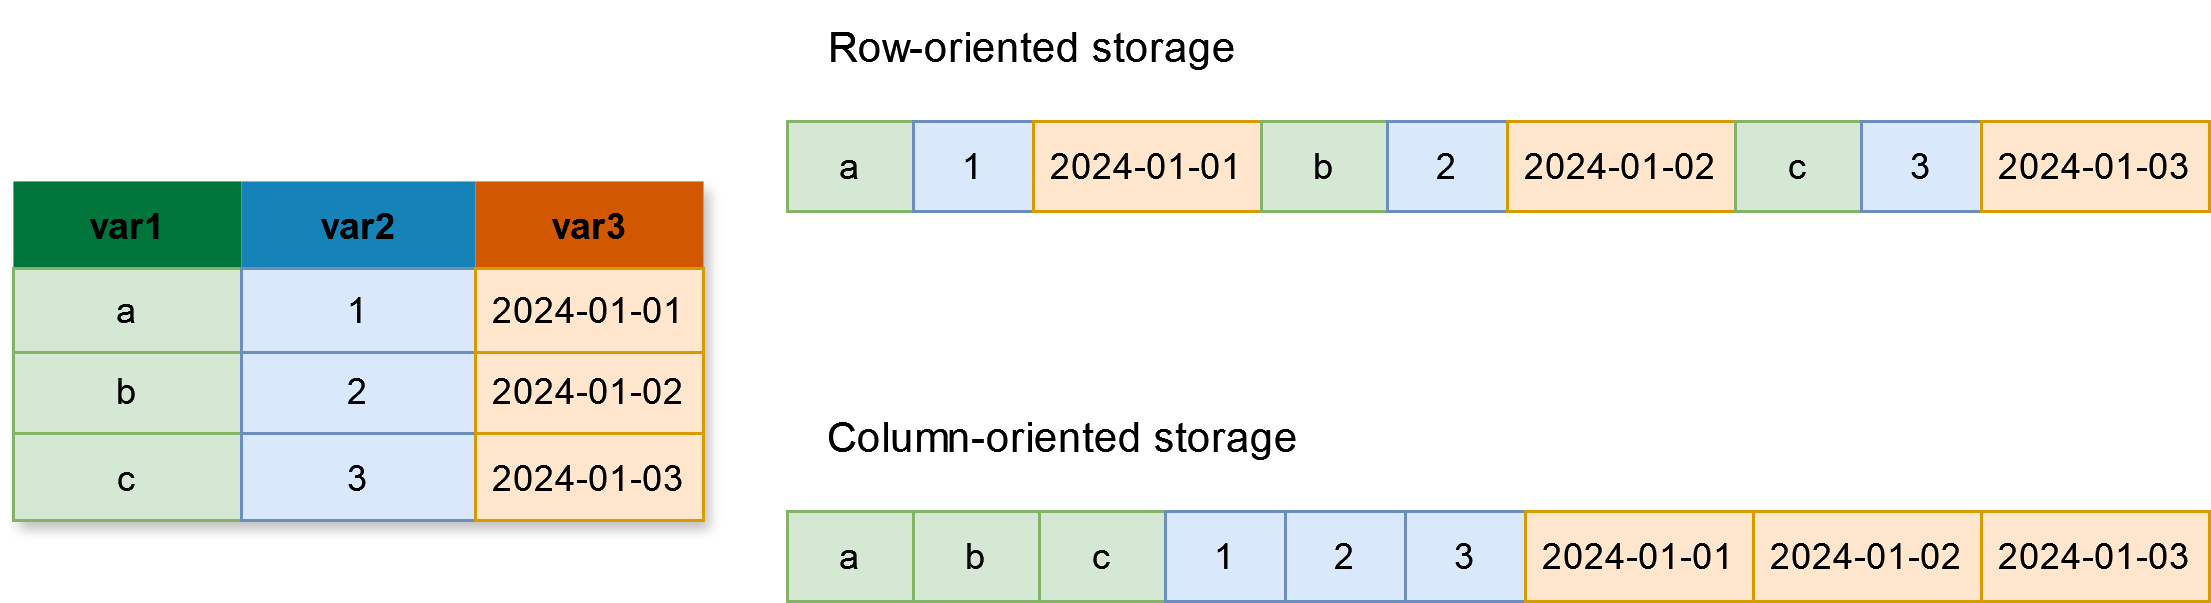
\includegraphics[width=\linewidth]{sections/img/columnar-storage.png}
    \caption{Row-oriented and column-oriented representation of a same dataset.}
    \label{fig:columnar-storage}
    \medskip
    {\footnotesize Note: Many statistical operations are analytical (OLAP) in nature: they involve selecting specific columns, computing new variables, performing group-based aggregations, etc. Row-oriented storage is not well-suited to analytical operations as it requires the full dataset to be read in memory to query it. Conversely, column-based storage allows only relevant data columns to be queried, significantly reducing read and processing times for analytical workloads. In practice, popular columnar formats such as Parquet use a hybrid-representation: they are primarily column-oriented but also implement clever row-based grouping to optimize filtering queries.}
\end{figure}

\subsection{Embracing cloud-native technologies}

In light of this evolution of the big data ecosystem, there has been a notable shift in recent years within the industry towards more flexible and loosely coupled architectures. The advent of cloud technologies has been instrumental in facilitating this shift. Unlike the era where Hadoop was prominent, network latency has become much less of a concern, making the traditional model of on-premise and co-located storage and compute solutions less relevant. In terms of the nature of the data that need to be processed, we are observing an evolution that some have described as moving "from big data to flexible data": modern data infrastructures are required not only to process large volumes but also to be adaptable in multiple dimensions: accommodating various data structures (ranging from structured, tabular formats to unstructured formats like text and images), ensuring data portability across multi-cloud and hybrid cloud environments, and supporting a diverse range of computational workloads (from parallel computations to deep learning models necessitating GPUs, as well as the deployment and management of applications) \cite{li2020big}. In recent years, two technologies have emerged in the data ecosystem as foundational technologies for achieving such flexibility in cloud-based environments: containerization and object storage. 

In a cloud environment, the computer of the user becomes a simple access point to perform computations on a central infrastructure. This enables both ubiquitous access to and scalability of the services, as it is easier to scale a central infrastructure — usually horizontally, i.e. by adding more servers. However, such centralized infrastructures have two well-identified limitations that need to be dealt with: the competition between users in access to physical resources and the need to properly isolate deployed applications. The choice of containerization is fundamental as it tackles these two issues \cite{bentaleb2022containerization}. By creating “bubbles” specific to each service, containers guarantee application isolation while remaining lightweight, as they share the support operating system with the host machine (see. graph\ref{fig:containers}). In order to manage multiple containerized applications in a systematic way, containerized infrastructures generally rely on an orchestrator software — the most prominent one being Kubernetes, an open-source project initially developed by Google to manage its numerous containerized workloads in production \cite{vano2023cloud}. Orchestrators automate the process of deploying, scaling, and managing containerized applications, coordinating their execution across various servers. Interestingly, this property makes it possible to handle very large volumes of data in a distributed way: containers break down big data processing operations into a multitude of small tasks, organized by the orchestrator. This minimizes the required resources while providing more flexibility than hadoop-based architectures \cite{zhang2018comparative}.

\begin{figure}[htbp]
    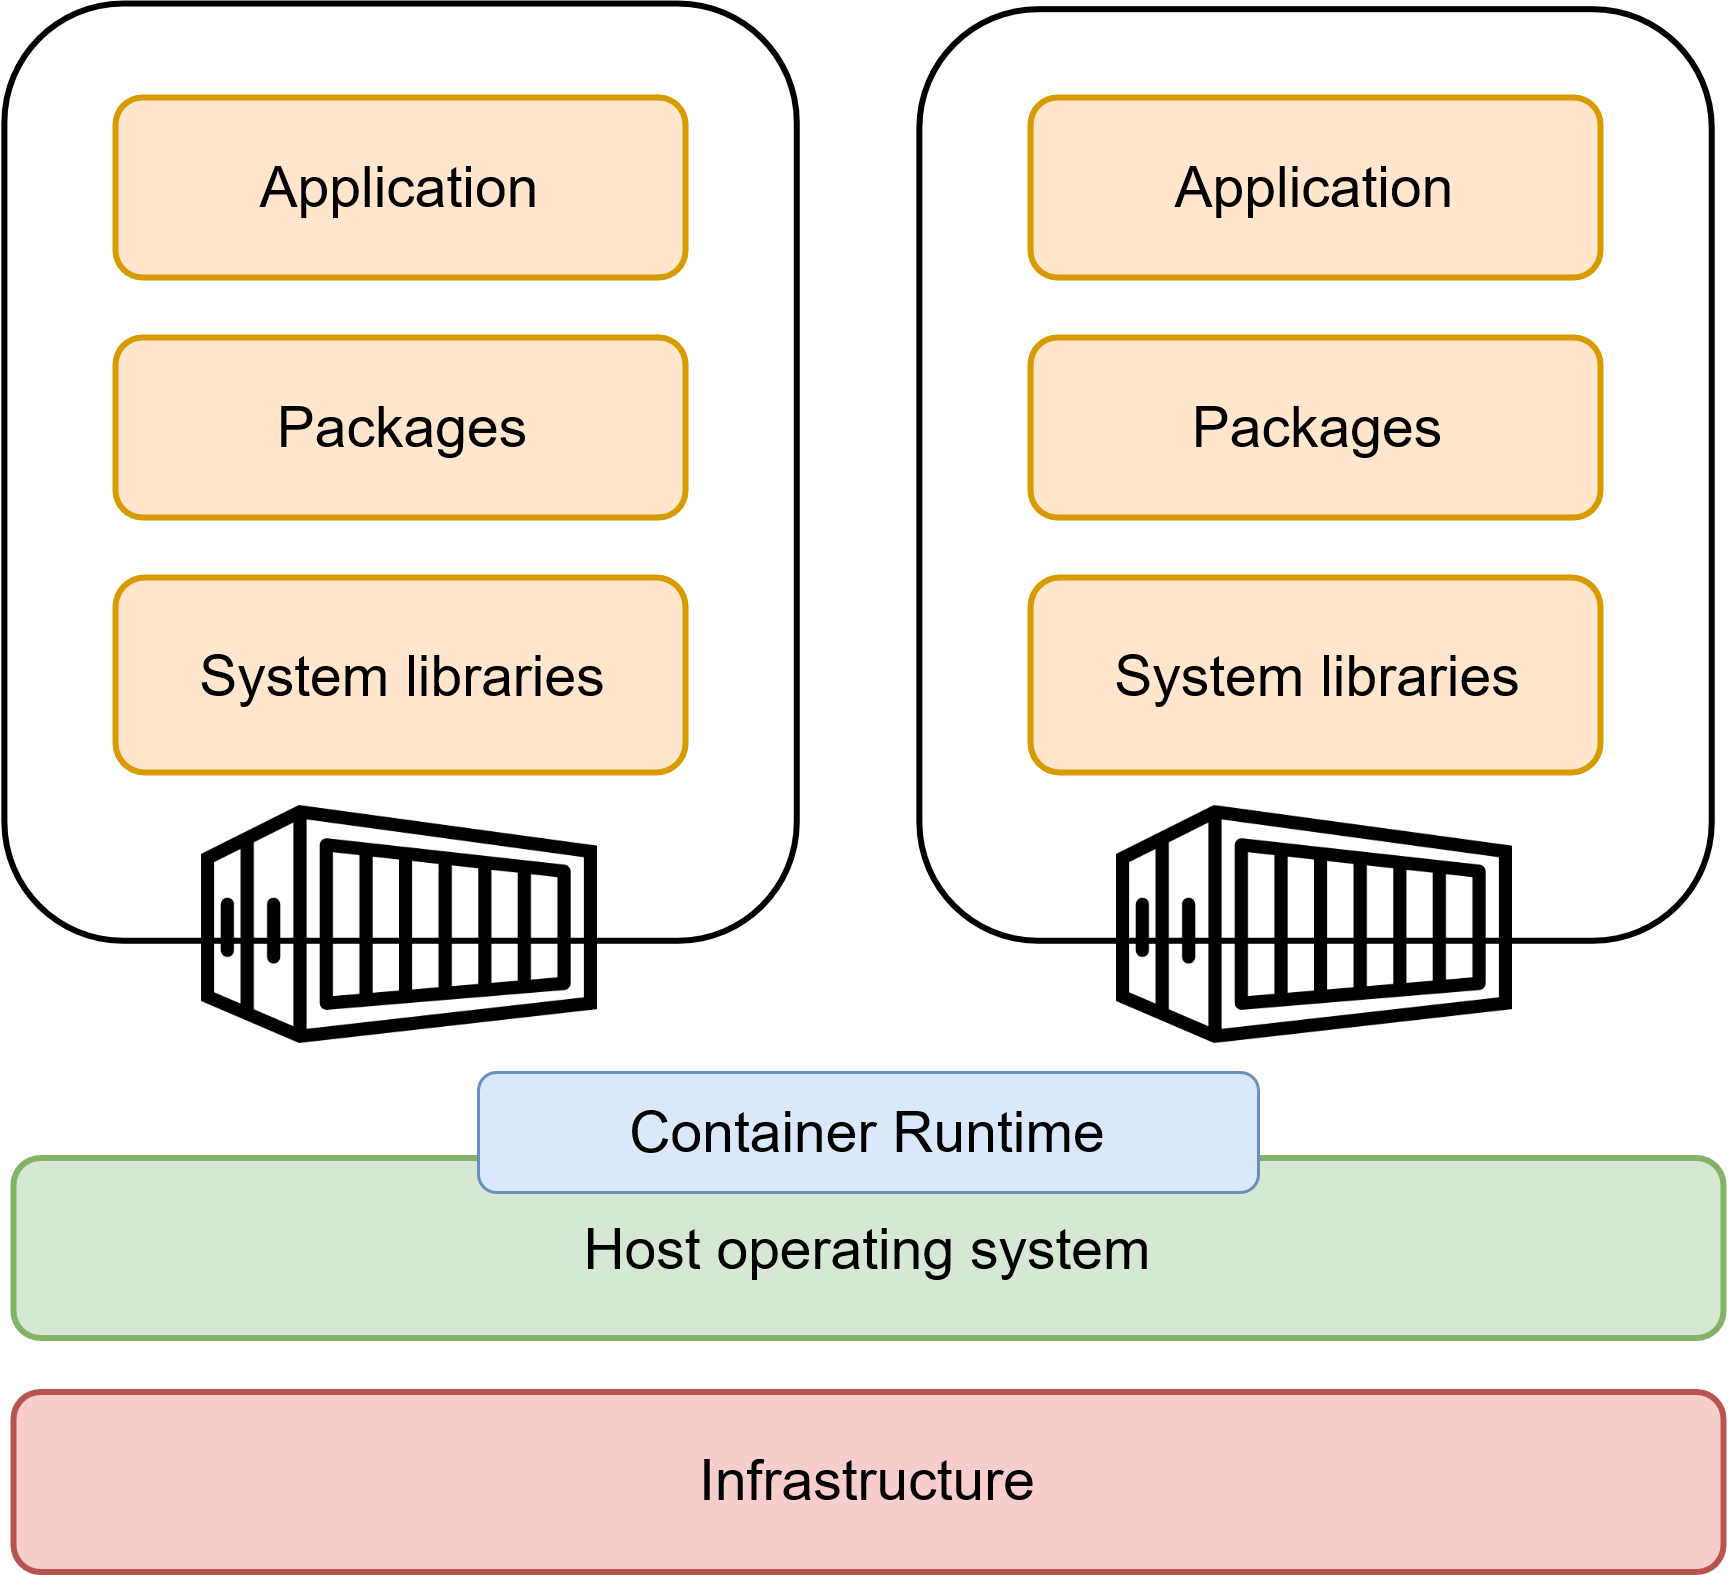
\includegraphics[width=\linewidth]{sections/img/containers.png}
    \caption{Architecture of a containerized environment.}
    \label{fig:containers}
    \medskip
    {\footnotesize Note: A container is a logical grouping of resources that makes it possible to encapsulate an application (e.g. Python code), the packages used (e.g. Pandas, NumPy) and system libraries (the Python interpreter, other OS-dependent libraries, etc.), in a single package. Containerized applications are isolated from one another through virtualization, which makes it possible to attribute specific physical resources to each application while guaranteeing complete independence between them. But contrary to virtual machines which also virtualize the operating system, containers rely on a lightweight form of virtualization: the operating system is shared with the host infrastructure. As a result, containers are much more portable and can be readily deployed and redistributed.}
\end{figure}

The other fundamental choice in a data architecture is the nature of data storage. In the cloud ecosystem, so-called "object storage" has become the de-facto reference \cite{samundiswary2017object} \footnote{Mainly because of Amazon's "S3" (Simple Storage Service) implementation.}. In this paradigm, files are stored as "objects" consisting of data, an identifier and metadata. This type of storage is optimized for scalability, as objects are not limited in size and the underlying technology enables cost-effective storage of (potentially very) large files. It is also instrumental in building a decoupled infrastructure such as discussed before: the data repositories — referred to as "buckets" — are directly searchable using standard HTTP requests through a standardized REST API. In a world where network latency is not the main bottleneck anymore, this means that storage and compute don't have to be on the same machines or even in the same location, and can thus scale independently according to specific organization demands. Finally, object storage is a natural complement to architectures based on containerized environments for which it provides a persistence layer — containers being stateless by design — and easy connectivity without compromising security, or even with strengthened security compared with a traditional storage system \cite{mesnier2003object}.

\subsection{Leveraging cloud technologies to increase autonomy and foster reproducibility}

Understanding how the technological choices described in the technical discussion above are relevant in the context of official statistics require an in-depth review of statisticians’ professional practices in their use of computing environments. At the end of the 2000s, with micro-computing at its peak, many of the technical resources used by statisticians at Insee were local: the code and processing software were located on individual computers, while data was accessed through a file-sharing system. Because of the the limited scalability of personal computers, this setup greatly limited the ability of statisticians to experiment with big data sources or computationally intensive statistical methods, and involved security risks because of the widespread data dissemination within the organization. In order to overcome these limitations, a transition was made towards centralised IT infrastructures, concentrating all — and thus overall much more — resources on central servers. Such infrastructures, made available to statisticians through a shared, virtual desktop environment for ease of use, remains the dominant method for conducting statistical computations at Insee at the time of writing this lines.

Through our observations and discussions with fellow statisticians, it became evident that although the current IT infrastructure adequately supported the core activities of statistical production, it noticeably restricted statisticians' capacity to experiment freely and innovate. The primary bottleneck in this organization is the dependency of statistical projects on centralized IT decision-making, such as the allocation of computing resources, access to shared data storage, the use of pre-configured programming languages and packaging environments, etc. Besides, such dependencies often lead to a well-known phenomenon within the software development community that lies at the heart of the DevOps approach, where the priorities of developers — iterate rapidly to improve functionality in a continuous manner — often clash with IT's focus on security and process stability. On the contrary, it is our understanding that modern data science practices reflect an increased involvement of statisticians in the IT development and orchestration of their data processing operations, beyond merely the design or validation phases. New data science infrastructures must take this expanded role of their users into account, giving them more autonomy than conventional infrastructures.

Cloud technologies stand out as a powerful solution to grant statisticians this much-needed autonomy in their daily work, enabling a culture of innovation. Through object storage, users gain control over the storage layer, allowing them to experiment with diverse datasets without being constrained by the limited storage spaces typically allocated by IT departments. Containerization empowers users to customize their working environments to their specific needs — be it programming languages, system libraries, or package versions — while also providing the flexibility to scale their applications according to the required computing power and storage capacities. By design, containers also foster the development of portable applications, which enables smoother transitions between environments (development, qualification, production), ensuring that applications can be moved seamlessly without the hurdles of environmental inconsistencies. Finally, with orchestration tools like Kubernetes, statisticians can more readily deploy applications and APIs and automatize the whole building process, sidestepping complexities associated with inconsistent or complex deployment environments. This capability aligns with the DevOps approach, enabling quicker iteration and building minimal prototypes as proofs of concept (POCs) rather than building the optimal (but time-consuming) solution for a pre-defined objective \cite{leite2019survey}.

% TODO: figure diagram object storage + compute -> reproductible outputs

Besides scalability and autonomy, these architectural choices also foster reproducibility of statistical computations. The concept of reproducibility — namely the ability to reproduce the result of an experiment by applying the same methodology to the same data — is a fundamental criterion of scientific validity \cite{mcnutt2014reproducibility}. It is also highly relevant in official statistics, as it serves as a foundation for transparency, which in turn is crucial for building and maintaining the public's trust. Fostering reproductibility in statistical production involves devising processing solutions that can produce reproducible statistics on the one hand, and that can be shared with peers on the other hand \cite{ntts2019reproducibility}. Traditional IT infrastructures — either a personal computer or a shared infrastructure with remote desktop access — fall short in this regard, as building a project or just computing a statistical indicator there generally involves a series of manual steps (installing system libraries, the programming language binary, projects packages, dealing with potentially conflicting versions, etc.) that can not be fully reproduced across projects. In comparison, containers are reproducible by design, as their build process involves defining precisely all the needed resources as a set of processing operations in a standardized manner, from the "bare machine" to the running application \cite{moreau2023containers}. Furthermore, these reproducible environments can be easily shared to peers as they can be readily published on open registries (for example, a container registry such as DockerHub) along to the source code of the application (for example, on a public software forge like GitHub or GitLab). This approach significantly enhances the reusability of code projects, fostering a community-driven model of development and innovation.


\label{sec:3}
\section{Onyxia: an open source project to build cloud-native data science platforms}



The Onyxia project, initiated by the French Public Service and available at
onyxia.sh, is an open source project aimed at creating self-sufficient data science environments in the cloud or on-premises. This project can be seen as a “Platform as a Package” (PaaP) solution for organisations wishing to create a data science environment based on cloud technologies.

\subsection{Making cloud-technologies accessible to statisticians}

Our technology watch and literature review highlighted cloud-native technologies, in particular containerization and object storage, as instrumental in building a data science platform that is both scalable and flexible. Building on these insights, we established our initial Kubernetes cluster in 2020, integrating it with MinIO, an open-source object storage system designed to work seamlessly with Kubernetes. Yet, our first experiments highlighted a significant barrier to their widespread adoption by statisticians: the complexity of their integration. This is an important insight when building data architectures in a modular fashion. By definition, this modularity lies at the source of the flexibility we are looking for - for instance, MinIO being compatible with the Amazon S3 API, the storage source could almost effortlessly be switched to a public cloud provider. However, it also means that any data application launched on the cluster must be configured so as to communicate with all the required components. For instance, in a big data setup, configuring Spark to operate on Kubernetes and interact with datasets stored in MinIO requires an intricate set of configurations (specifying endpoints, access tokens, etc.), a skill set that typically lies beyond the expertise of statisticians.



Axe : mise à dispo des technos cloud $\rightarrow$ favoriser l'autonomie.
- convergence des choix d'archi. Mais suffisant pour garantir l'autonomie : non $\rightarrow$ les outils de l'éco-système s'adressent plutôt à des informaticiens (ex : difficulté de configurer Spark sur du stockage objet en mode kube)
- Eco système découplé, mais exigeant $\rightarrow$ compétences diverses.
- Enjeu : faciliter l'acces aux ressources cloud pour les statisticiens (qui doit déjà s'acculturer à la reproductibilité $\rightarrow$ convergence avec les outils des développeurs) $\rightarrow$ double décalage qui demande une assistance
- IHM Onyxia comme liant technique

\subsection{Architecture principles aimed at fostering autonomy}

- no vendor-lockin (enfermement de la structure $\rightarrow$ coût (licences) et des pratiques $\rightarrow$ fige les compétences)

Another significant risk with commercial cloud services is vendor lock-in
(Opara-Martins, Sahandi, and Tian 2016). Organisations may become increas-
ingly integrated with the tools and services of one cloud provider, potentially
making transitions to other platforms difficult and resource-intensive. This de-
pendency can restrict adaptability and might increase operational costs over
time. Recognizing these challenges, there is a trend towards endorsing cloud-
neutral strategies (Opara-Martins, Sahandi, and Tian 2017). These methods
aim to engage with cloud services in a way that reduces reliance on a single
vendor’s specific solutions.

- cloud-native : onyxia n'est pas le choix fondamental, le parti pris est sur le choix sous-jacent : conteneurisation + stockage objet
- Acculturation aux bonnes pratiques par l'usage

\subsection{An extensive catalogue of services to cover the entire lifecycle of data science projects}

Axe : principes
- A catalog of services which covers the entire lifecycle of a data science project
- production-ready : outils d'automatisation (-> autonomie)

\subsection{Building commons : an open-source project and an open-innovation platform}

- Orientation plateforme : instance vivante d'Onyxia, ouverte, collaborative, sandbox (cf. ref papier SSP Cloud sur l'aspect plateforme)
- Innovation ouverte $\rightarrow$ littérature
- Open-data
- Instance de partage : formations reproductibles + utilisation dans les écoles de stats + hackathons (organisation annuelle du funathon cf. one-stop-shop)


\label{sec:4}
\section{Case-study : using MLOps to improve NACE classification}
\label{sec:mlops}

This chapter aims, through a concrete example, to illustrate how Insee managed to deploy its first machine learning (ML) model into production. It will provide an in-depth description of the MLOps approach that this project strived to adhere to, focusing on the various technologies that were employed. In particular, we will highlight how cloud technologies were instrumental in building a solution iteratively and how Onyxia greatly facilitated this process by providing flexible development environments as well as tools to deploy and monitor models, promoting a continuous improvement loop. The entire project is available in open source\footnote{\url{https://github.com/orgs/InseeFrLab/teams/codification-ape/repositories}} and remains under active development.






\subsection{Improving the NACE classification process using ML methods}

\subsubsection{Motivation}

Coding tasks are common operations for NSOs and can sometimes be challenging due to the size of nomenclatures. At Insee, a sophisticated coding tool called Sicore was developed in the 1990s to perform various classification tasks. It consists in a coding engine containing a large number of deterministic rules which identify ground-truth labels. Each input label goes through these rules and when a ground-truth label is recognized, the associated code is assigned. When the label is not recognized, it must be manually classified by an Insee agent. 

Two main reasons drove the experimentation of new coding methods. Firstly, there was an internal change with the redesign of the Sirene registry, which lists all companies in France and assigns them a unique identifier, the Siren number, used by public institutions. The main goals of this revamping were to improve the daily management of the registry for Insee agents and to reduce waiting times for companies. Additionally, at the national level, the government launched a one-stop shop for business formalities, allowing more flexibility for business owners in describing their main activities. Initial testing exercises revealed that Sicore was no longer the suitable tool for performing NACE classification, as only 30\% of the input data were being automatically coded.

Three stakeholders were involved in this project: the \textit{business team}\footnote{We refer to the business team, the team that has business knowledge i.e. who knows the NACE perfectly.} responsible for managing the Sirene registry, the \textit{IT team} developing software related to the registry's operation, and the \textit{innovation team} responsible for implementing the new coding tool. The latter team is the Insee Lab, which was created in 2017 with the objective of providing support to other teams on innovation topics to streamline their various projects.

\subsubsection{Classification task}

The project we are describing consists in a standard NLP classification problem. Starting from a textual description of the activity, we want to predict the associated class in the NACE Rev. 2 nomenclature. This nomenclature has the particularity of being hierarchical and contains 5 different levels\footnote{Actually, there are 5 different levels in France but only 4 at the European level.}: section, division, group, class, and subclass. In total, 732 subclasses are included in the nomenclature, which is the level at which we aim to perform the classification. Table \ref{tab:nace-nomenclature} provides an example of this hierarchical structure.

\begin{table}[htbp]
    \centering
    \begin{tabular}{llll}
    \textbf{Level} & \textbf{NACE} & \textbf{Title} & \textbf{Size} \\ \hline
    Section & H & Transportation and storage & 21 \\ \hline
    Division & 52 & Warehousing and support activities for transportation & 88 \\ \hline
    Group & 522 & Support activities for transportation & 272 \\ \hline
    Class & 5224 & Cargo handling & 615 \\ \hline
    \textbf{Subclass} & \textbf{\textcolor{red}{5224A}} & \textbf{Harbour handling} & \textbf{\textcolor{red}{732}} \\ 
    \end{tabular}
    \caption{NACE Nomenclature}
    \label{tab:nace-nomenclature}
    \end{table}

With the establishment of the one-stop shop, business owners now describe their activity description with a free-text field. As a result, the new labels are very different from the harmonized labels that were previously received. Therefore, it was decided to work with ML models, that are known to be effective on supervised text classification tasks \cite{li2022survey}. This represents a significant paradigm shift from Insee's perspective, as ML was not traditionally used in the actual production of official statistics. Besides, the perspective of putting the new model in production was considered from the outset, guiding numerous methodological and technical choices. As such, several strategic choices had to be made from the outset, including the methodology, the choice of a development environment consistent with the target production environment, and the adoption of collaborative work methods.

\subsubsection{Methodology}

Text classification from the free-text field provided by business owners is a complex task: the activity descriptions are relatively short and thus contain limited statistical information, can contain spelling mistakes, and often require domain knowledge to be properly classified. On such task, traditional text analysis methods such as count vectorization or TF-IDF often fall short whereas neural-network-based embedding methods tend to perform better \cite{li2022survey}. However, such architectures impose greater demands on the production setting, as they are much larger and often require specific hardware such as GPUs to be fine-tuned and perform inference with acceptable latency. These constraints led us away from the most powerful language models, such as Transformer models, and instead directed us towards the fastText model \cite{joulin2016bag}, a simpler embedding-based classifier. The fastText model is extremely fast to train, even from scratch, and inference doesn't require a GPU to achieve low latency time. Besides, the model yielded excellent performance results for our use-case which, considering the time and human resource constraints, were more than sufficient to enhance the existing process. Finally, the model's architecture is relatively simple, which simplified communication and adoption within the various Insee teams.

The fastText model relies on a bag-of-words model to obtain embeddings and a classification layer based on logistic regression. The bag-of-words approach involves representing a text as the set of vector representations of each of its constituent tokens. With FastText, the embedding of a sentence is computed as a function of the individual embeddings, typically the average. In the case of supervised text classification, the embedding matrix and the classifier's parameters are learned simultaneously during training by gradient descent, minimizing the cross-entropy loss function. The specificity of the fastText model compared to other embeddings-based approaches is that embeddings are not only computed on words but also on word n-grams and character n-grams, providing more context and reducing biases due to spelling mistakes. Figure \ref{fig:fasttext} represents the full pipeline of operations performed by fastText on an example text input.

\begin{figure}[htbp]
    \centering
    \makebox[\textwidth][c]{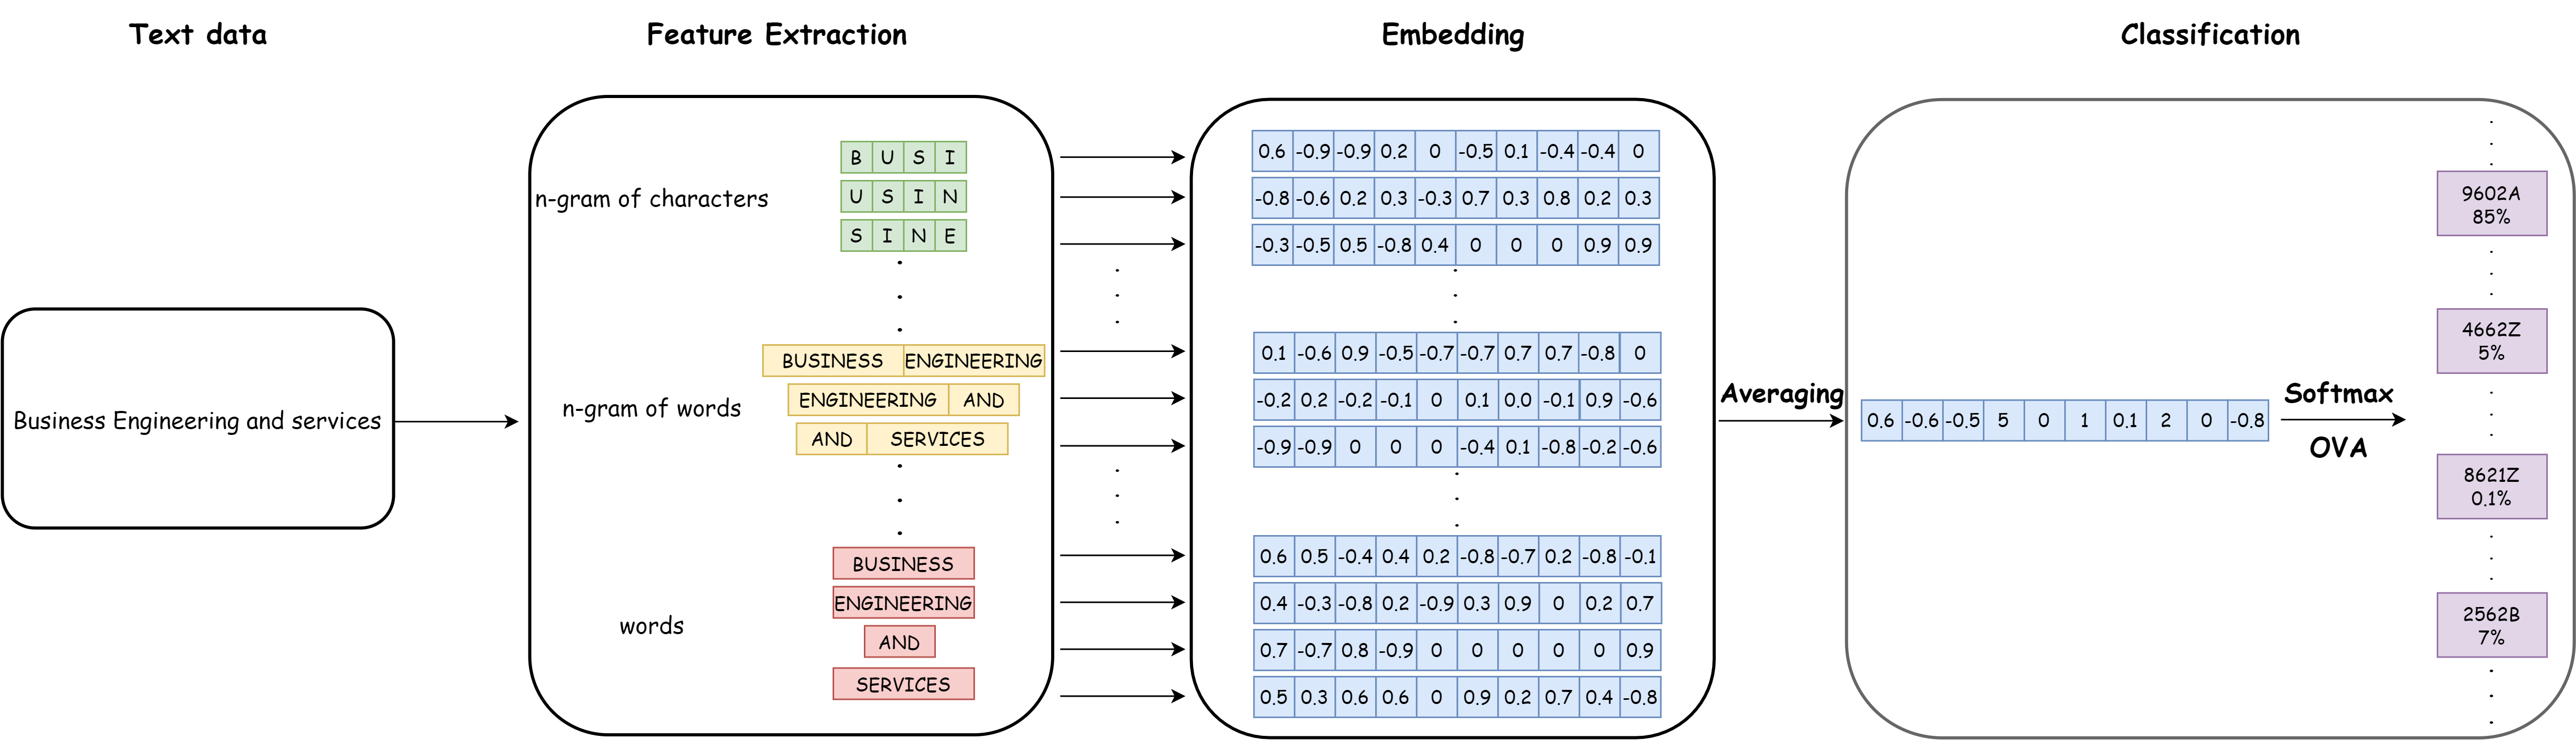
\includegraphics[width=1.5\textwidth]{sections/img/fasttext.png}}
    \caption{Simplified architecture of the fastText model}
    \label{fig:fasttext}
\end{figure}






\subsection{A production-first approach with MLOps}

From the very onset of this project, the target was to go beyond mere experimentation and put the model in production. Besides, the goal with this pilot project was also to build a template for future ML projects at Insee. We thus strove to enforce best development practices from the very beginning of the project: following community standards for code quality, using scripts-based development over notebooks, building a modular package-like structure, etc. However, compared to traditional development projects, machine learning projects have specific features that make it necessary to apply a complementary set of best practices, gathered under the name of MLOps.

\subsubsection{From DevOps to MLOps}
\label{subsubsec:devops-mlops}

DevOps is a set of practices designed to foster collaboration between development (Dev) and operations (Ops) teams. The fundamental idea is to integrate the full lifecycle of a project in a single automated continuum. An important tool to achieve this continuity is CI/CD pipelines. With continuous integration (CI), each commit of new source code will trigger a pipeline of standardized operations, such as building the application, testing it and making it available as a release. Then, continuous deployment (CD) consists in tools to automate the deployment of the new code and limit manual intervention, while ensuring proper monitoring to guarantee process stability and security. This approach promotes a more rapid, continual release of necessary feature changes or additions. Furthermore, by encouraging collaboration between teams, DevOps also promotes a quicker cycle of innovation, allowing teams to address issues as they arise and incorporate feedback effectively throughout the project lifecycle.

The MLOps approach can be seen as an extension of DevOps, developed to address the specific challenges related to managing the lifecycle of ML models. Fundamentally, both DevOps and MLOps aim at building software in a more automated and robust manner. The main difference is that in MLOps, this software also has a machine learning component. Consequently, the lifecycle of the project gets more complex. The underlying ML model needs to be trained, often periodically in order to prevent potential performance losses over time. Data ingestion must also be included in the pipeline, as new data may be used to improve performance. Figure~\ref{fig:mlops-cycle} presents the steps of a ML project using the continuous representation traditionally seen in DevOps. This illustrates a fundamental principle of MLOps, the need for continuous improvement, described in more details in section~\ref{sec:principles-mlops}.

\begin{figure}[htbp]
    \centering
    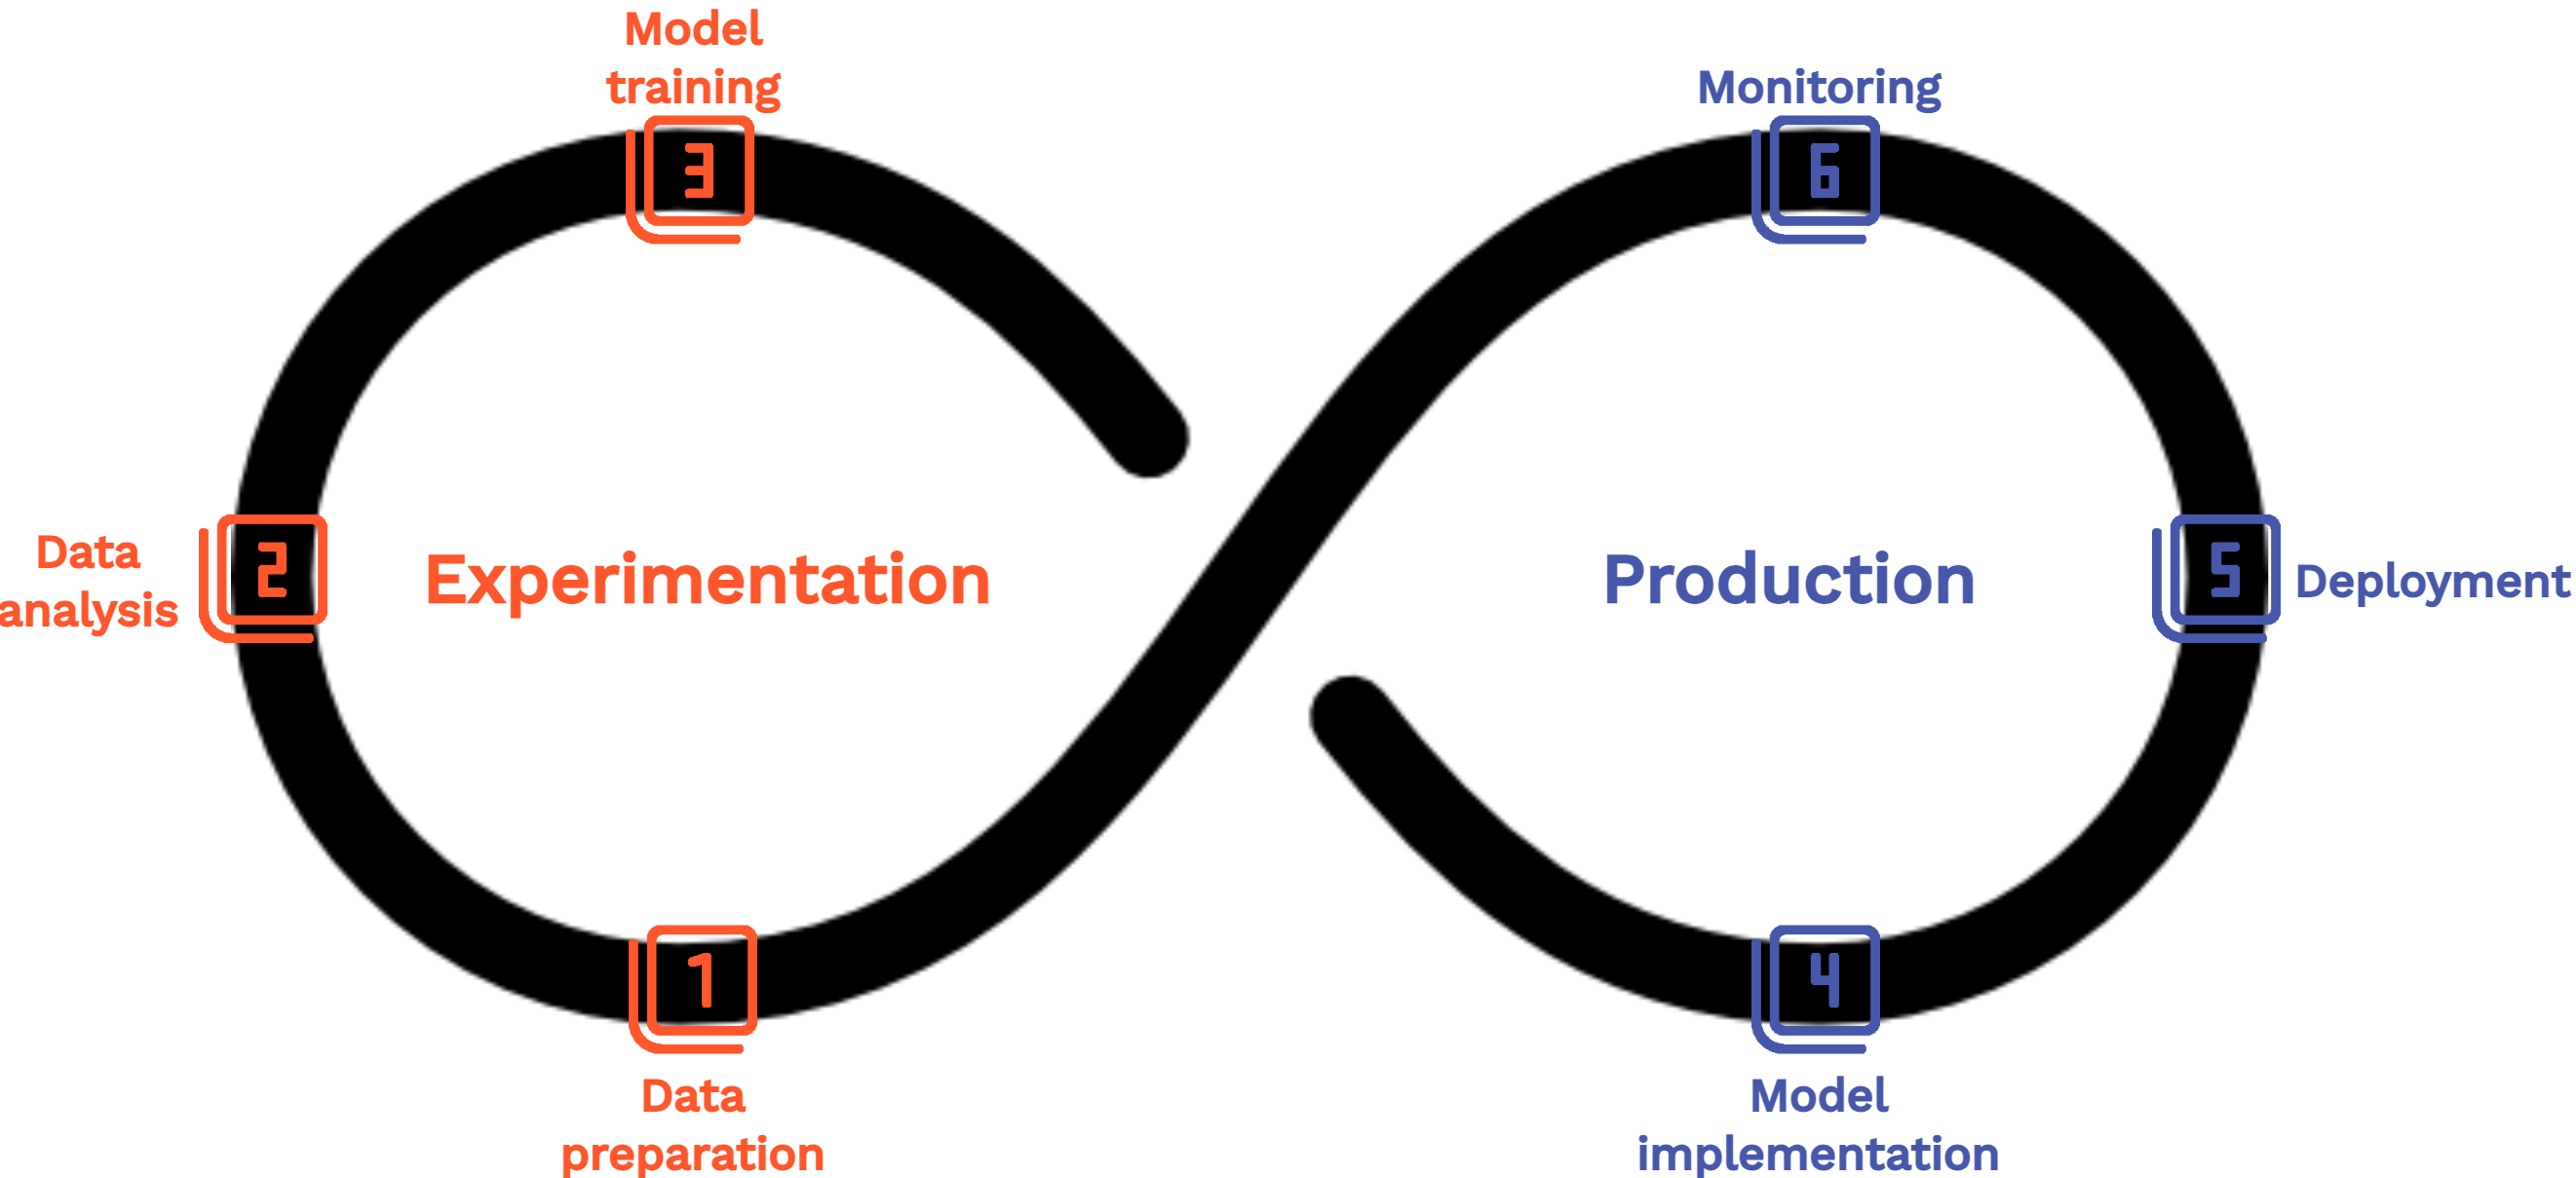
\includegraphics[width=\textwidth]{sections/img/mlops-cycle.png}
    \caption{The MLOps approach promotes a continuous management of ML projects lifecycle}
    \label{fig:mlops-cycle}
\end{figure}

\subsubsection{Principles of MLOps}
\label{sec:principles-mlops}

MLOps is defined by a few core principles that are crucial for building production-ready and scalable ML applications. These principles are designed to address the specific challenges associated with ML workflows.

The most fundamental principle of MLOps is continuous improvement, in order to reflect the iterative nature of ML projects. In the experimentation phase, the model is developed using a training dataset, which will generally differ somewhat from the target data. When a model is deployed in production, the new data that the model needs to perform prediction one can reveal insights about the model's performance and potential shortcomings. These insights necessitate a return to the experimentation phase, where data scientists adjust or redesign their models to address any discovered issues or to improve accuracy. This principle thus emphasizes the importance of building a feedback loop that enables ongoing enhancements throughout the lifecycle of a model. Automation, particularly through the use of CI/CD pipelines, plays a crucial role in this process by making the transition between experimentation and production phases more continuous. Monitoring is also an essential part of this process: a model deployed in production needs to be continuously assessed so as to detect data or concept drifts that may reduce the predictive performance of the model and thus necessitate further adjustments, such as re-training  or fine-tuning the model.

Another major goal of MLOps is to promote reproducibility, which ensures that any ML experiment can be reliably repeated and will produce the same results. MLOps tools thus facilitate thorough logging of ML experiments, including data pre-processing steps, model hyper-parameters, and training algorithms. Data, models, and code are versioned, enabling teams to revert to previous versions if an update does not perform as expected. Finally, these tools help producing detailed specifications of the computing environment used to produce these experiments — such as versions of libraries — and often rely on containers to help replicate the same conditions in which the original model was developed.

Finally, MLOps aims at fostering collaborative work. ML-based projects generally involve a wider range of profiles: business units and data science teams on the one hand, developers and operations teams on the other. Like DevOps, MLOps thus emphasizes the need for a collaborative culture and to avoid working in silos. MLOps tools generally include collaborative features, such as centralized stores for ML models or ML features which facilitate the sharing of components between team members and limit redundancy.

\subsubsection{Implementation with MLFlow}

Numerous tools have been developed to implement the MLOps approach in actual projects. All of these frameworks aim at enforcing, in some form, the core principles described above. In this project, we chose to rely on a popular open-source framework named MLFlow\footnote{\url{https://github.com/MLflow/MLflow}}. This choice doesn't indicate any inherent superiority of MLFlow over alternative software, but reflects a set of good properties associated with MLFlow that made it a very relevant solution for our application. First, it is Kubernetes-native, reflecting our choice of the underlying infrastructure for the project. Second, it aims at covering the entire lifecycle of ML projects, while other tools may be more specialised in some parts of it. Third, it exhibits great interoperability as it is well-interfaced with with popular ML libraries — such as PyTorch, Scikit-learn, XGBoost, etc. — and supports multiple programming languages — including Python, R, and Java, thus covering the spectrum of programming languages copmmonly used at Insee. Finally, it proved to be very user-friendly and thus encouraged adoption among the project members and facilitated continuous collaboration between them.

MLFlow provides a cohesive framework to operationalize MLOps principles effectively within ML projects. Data scientists can encapsulate their work in MLFlow Projects, which package ML code and its dependencies, ensuring that each project is reproducible and can be consistently re-executed. A project relies on an MLFlow Model, a standard format that is compatible with most ML libraries and offers a normalized way of serving the model, e.g. via an API. This interoperability and standardization are instrumental in supporting continuous improvement of the project, as models trained with a variety of packages can be readily compared or switched by one another without breaking any code. As experiments with various models progress, the Tracking Server logs detailed information about each run — hyper-parameters, metrics, and outputs artifacts and metrics — which there again promotes reproducibility but also facilitates the model selection phase through a user-friendly interface. After this experimentation phase, selected models are integrated into the Model Registry, where they are versioned and staged for deployment. This registry serves as a centralized model store that enables the different project members or teams to collaboratively manage the lifecycle of the project. Figure~\ref{fig:mlflow-components} shows the core components of MLFlow and how they facilitate a more continuous and collaborative workflow inside a ML project.

\begin{figure}[htbp]
    \centering
    \makebox[\textwidth][c]{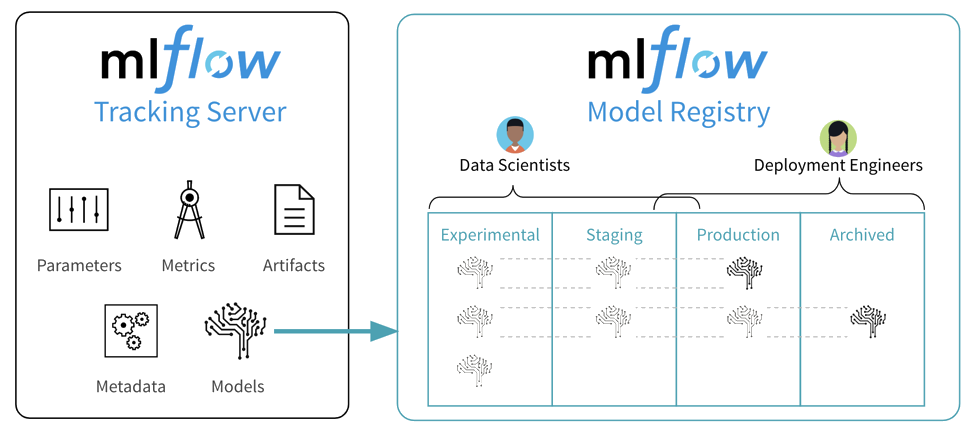
\includegraphics[width=\textwidth]{sections/img/mlflow-model-registry.png}}
    \caption{Core components of MLFlow. Source: Databricks.}
    \label{fig:mlflow-components}
\end{figure}






\subsection{Leveraging cloud technologies to foster iterative development}

While continuous improvement is a fundamental principle of MLOps, it is also a very demanding one. In particular, it requires to design and build our project as an integrated pipeline whose various stages are mainly automated, from data ingestion to monitoring the model in production. In this context, iterative development is essential in order to build a minimum viable product that is then refined over time. This section aims to show how cloud-native technologies, through the Onyxia project, were instrumental in building the project from the start as a collection of modular connected components, thus greatly enhancing the capacity for continuous refinement over time.

\subsubsection{A flexible development environment}

In a ML project, the flexibility of the development environment is essential. First, due to the diversity of tasks to be performed — data collection, preprocessing, modeling, evaluation, inference, monitoring, etc. Second, because ML is a fast-evolving field, it is preferable to build a ML app as a collection of modular components so as to be able to update components without disrupting the entire pipeline. As discussed in section~\ref{sec:cloud-native}, cloud-native technologies enable the creation of modular and scalable development environments.

However, as also discussed in section~\ref{sec:implementation}, access to such resources is not enough. A ML project that is developed following MLOps principles requires a wide variety of tools — data storage, interactive development environments to experiment freely, automation tools, monitoring tools, etc. While these tools can be installed on a Kubernetes cluster, making them available to data scientists in an integrated and pre-configured manner is essential to facilitate their adoption. Through its catalog of services and the automatic injection of configuration in the services, Onyxia enables building projects that rely on multiple cloud-native components that can communicate readily with each other.

The way model training was carried out for this project emphasizes the flexibility provided by Onyxia in the experimentation phase. All the code performing the training is written in Python in the context of a VSCode service. As personal S3 credentials are injected in each service at startup, the various users of the projects can interact directly with the training data stored on a S3 bucket on MinIO, Onyxia's default object storage solution. All experiments performed for the model selection phase are logged on a shared instance of MLFlow, which stores logged data on a PostgreSQL instance automatically launched on Kubernetes and artifacts (trained models and associated metadata) on MinIO. The model was trained using grid-search for hyperparameter tuning and evaluated through cross-validation, a combination that is known to provide a better evaluation of the generalization performance of the model but also requires a lot of computing resources, due to the combinatory nature of testing many hyperparameters combinations. In our case, we leveraged Argo Workflows, an open-source workflow engine designed to orchestrate parallel jobs on Kubernetes, each job being specified as an independent container. It then becomes straightforward to compare performances of the different trained models and select the best one using the comparison and visualization tools available in the UI of MLFlow. 

In summary, the training stage was made efficient and reproducible thanks to the use of numerous modularly connected components — a distinctive feature of cloud-native technologies — readily made available to data scientists by Onyxia.

\subsubsection{Deploying a model}

Once candidate models have been optimized, evaluated and a best-performing model has been selected, the next step is to make it available to the application end users. Simply providing the trained model as an artifact or even just the code to train the model is not a convenient way to serve it, as it assumes that users have the resources, infrastructure, and knowledge required for training it under the same conditions. The goal is therefore to make the model available in a simple and interoperable manner, in the sense that it should be possible to query it with various programming languages. Furthermore, it should be possible for other applications to query the model in a programmatic way. 

Against that background, we opted to serve the model through a REST API. This technology has become a standard way to serve ML models as they offer several benefits. First, they fit very well a cloud-oriented environment: similarly to the other components of our stack, it makes it possible to query the model using standard HTTP requests, which contributes to the modularity of the system. It also means that they are interoperable: as they rely on standards technologies for queries (HTTP requests) and responses (generally, a JSON-formatted string), they are mostly agnostic to the programming language used to request them. Finally, they offer great scalability because of their stateless design. As each request must contain all the information needed to understand and process the request, REST APIs can easily be duplicated on different machines to balance a challenging load — a process known as horizontal scaling.

To develop the API that serves the model, we used FastAPI\footnote{\url{https://fastapi.tiangolo.com}}, a fast and well-documented web framework for building APIs with Python. The API code and required software dependencies are encapsulated into a Docker image so that it can be deployed as a container on the Kubernetes cluster. An important benefit of using Kubernetes is the ability to scale the API — through the number of API pods effectively deployed — to the demand and provide automatic load-balancing. Upon startup, the API automatically retrieves the correct model from the MLflow model registry, which acts as a proxy from the actual artifact of the production model, stored on MinIO. Using a MLflow model enables to integrate the pre-processing step before each prediction to the API, greatly simplifying inference regardless of the ML framework used. This deployment process is summarized in Figure \ref{fig:api-datalab}.

\begin{figure}[htbp]
    \centering
    \makebox[\textwidth][c]{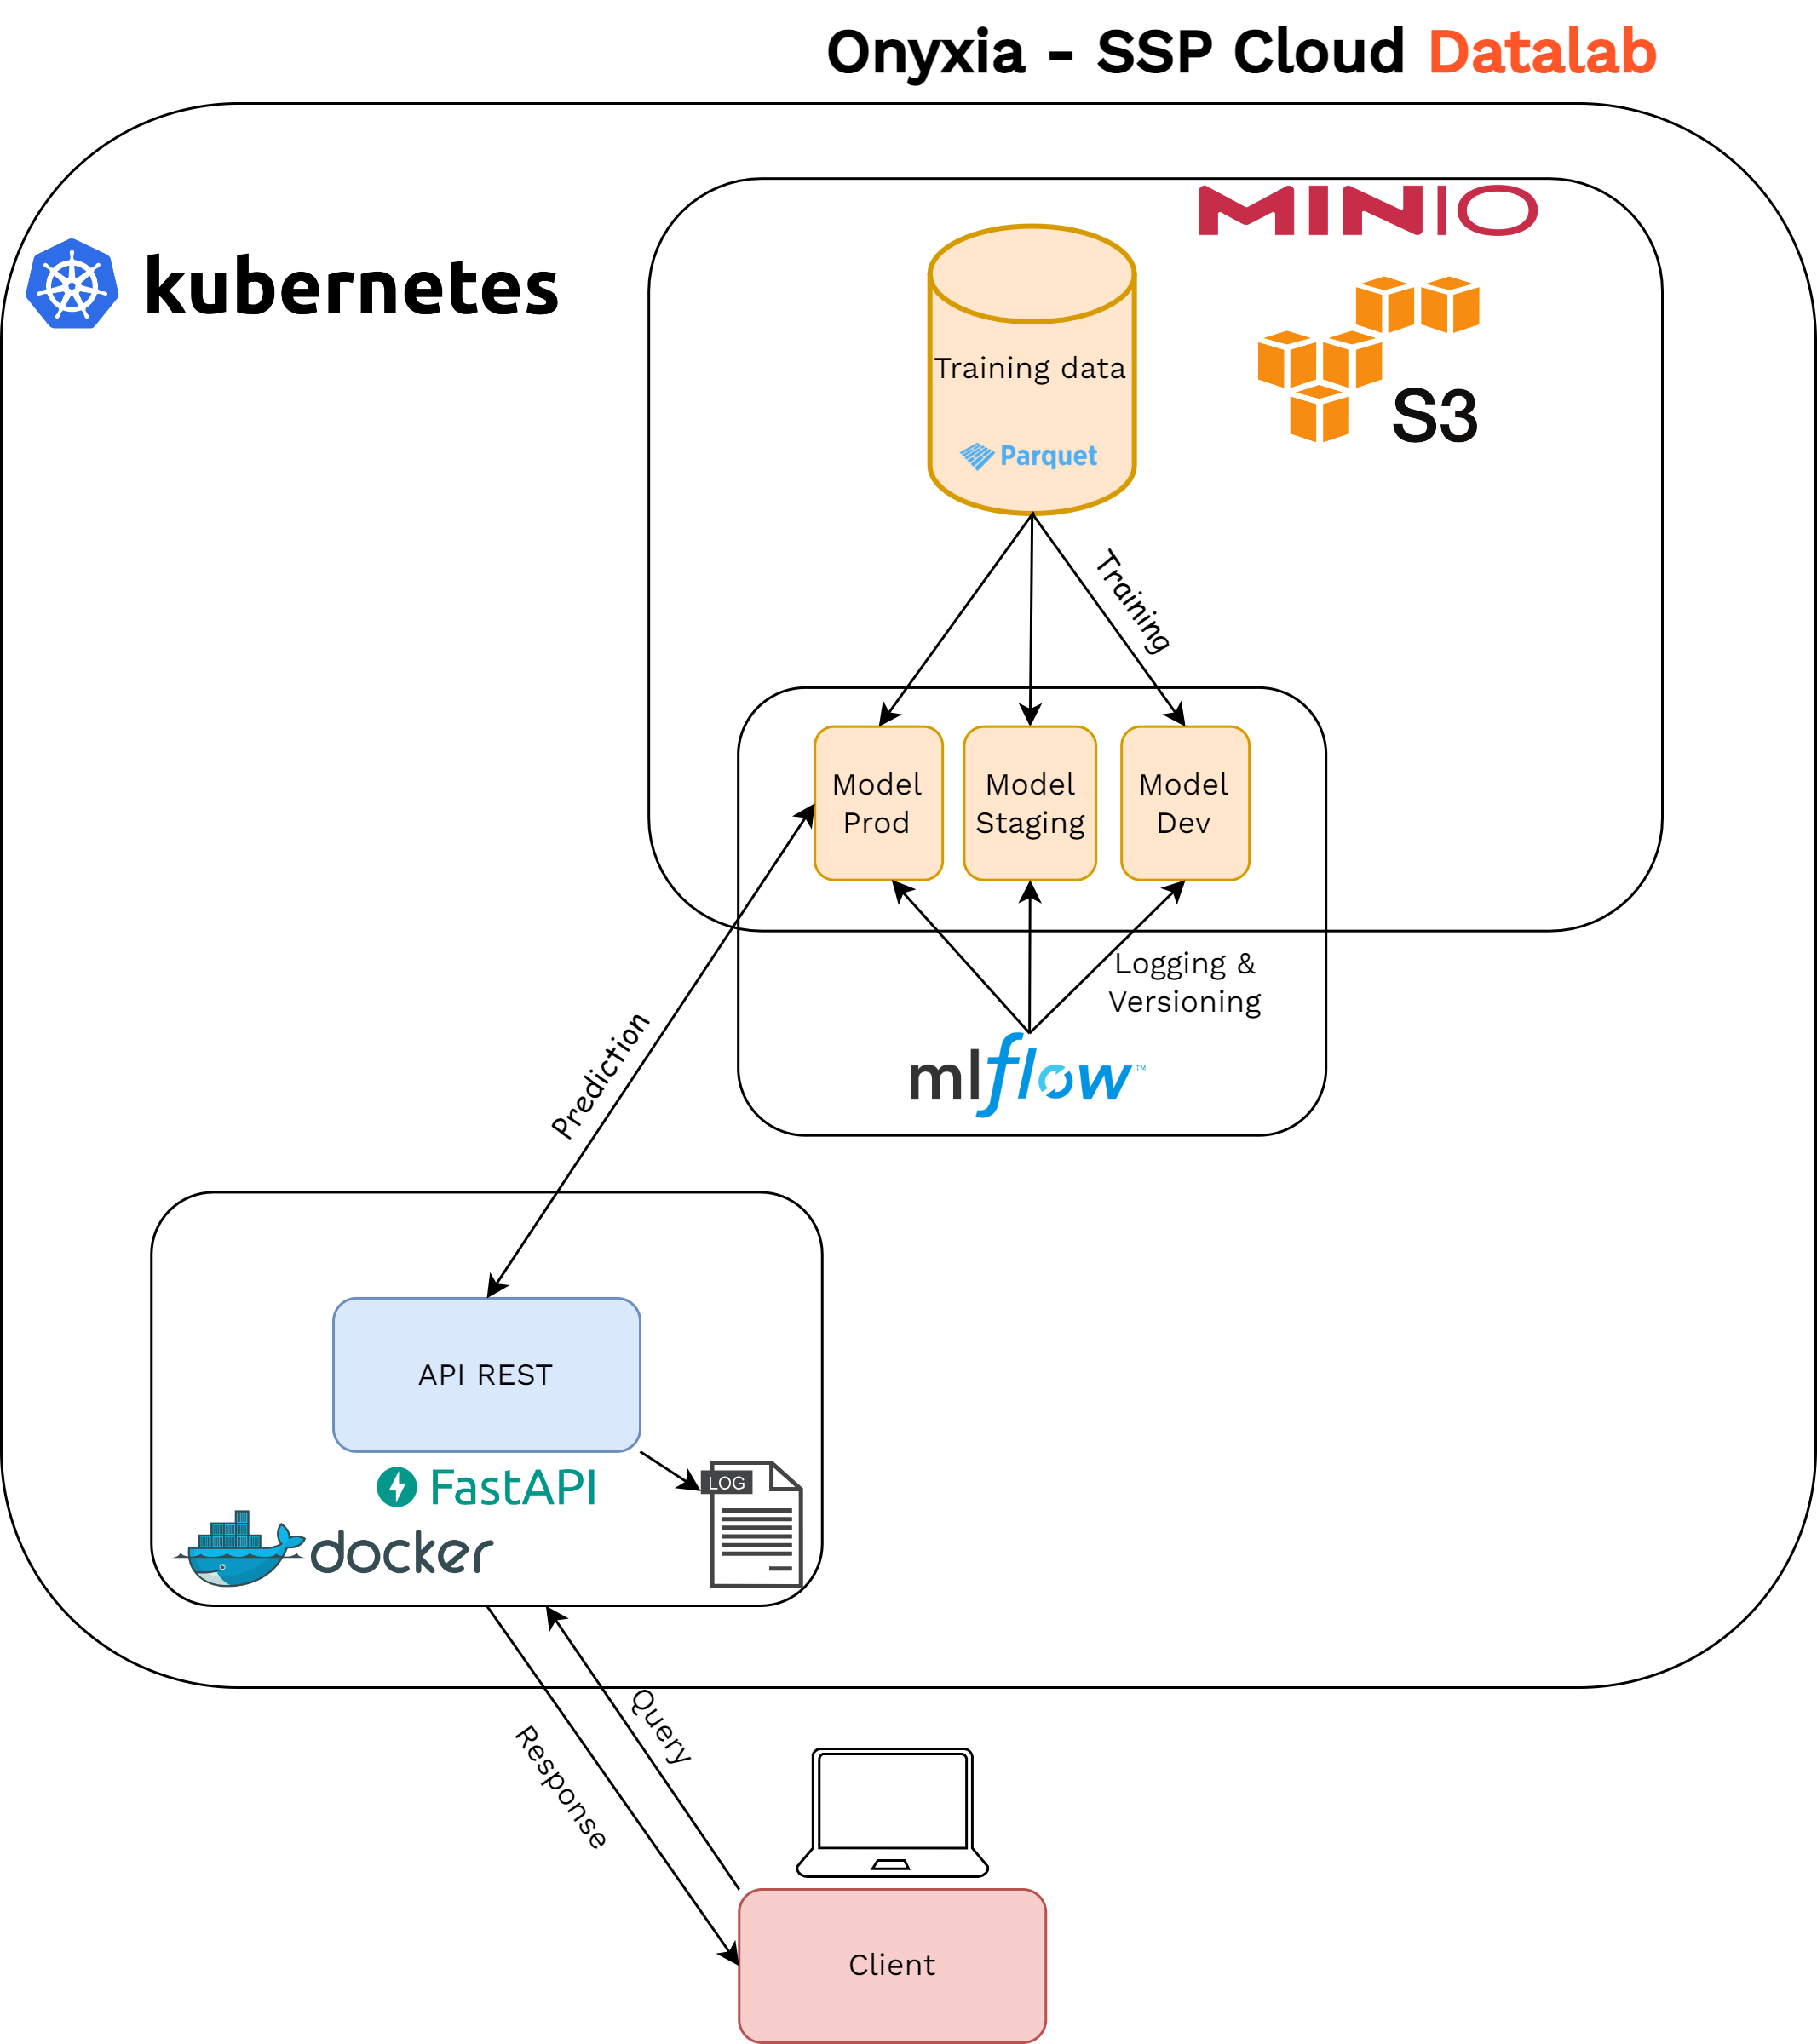
\includegraphics[width=0.75\textwidth]{sections/img/api-datalab.png}}
    \caption{A cloud-native approach to serve a ML Model using a REST API}
    \label{fig:api-datalab}
\end{figure}

\subsubsection{Building an integrated pipeline}

The architecture we built at this stage already reflects some important principles of MLOps. The use of containerization to deploy the API as well as the use of MLFlow to track the experiments while developing the model ensures reproducibility of the predictions. Using the central model registry provided by MLFlow facilitates the management of the lifecycle of the models in a collaborative way. Furthermore, the modularity of our architecture leaves room for further improvement as modular components can be easily added or modified without breaking the structure of the application as a whole. As we shall see in subsequent sections, this property was essential in building the application iteratively, enabling to add a monitoring layer (Section~\ref{subsubsec:monitoring}) and an annotation component (Section~\ref{subsubsec:annotation}) to promote continuous improvement of the model.

However, the ability to refine the base architecture iteratively also requires more continuity in the process. At this stage, the deployment process involves several manual operations. For instance, adding a new feature to the API would require to build a new image, tag it, update the Kubernetes manifests used to deploy the API and enforce them on the cluster to replace the existing one with minimum downtime. Similarly, a change of the model served through the API would require a very simple modification of the code but several manual steps to update the version on the cluster. As a result, data scientists are not fully autonomous when it comes to prototyping and testing updated versions of the model or the API, which limit the potential for continuous improvement.

In order to automate this process, we built a CI/CD pipeline — a concept already presented in Section~\ref{subsubsec:devops-mlops}) — integrating these various steps. Figure \ref{fig:ci-cd} illustrates our specific implementation of a CI/CD pipeline. Any change in the code of the API repository triggers a CI build process (implemented with GitHub Actions) of the associated docker image, which is then released on a public container registry (DockerHub). This image can then be fetched and deployed by the container orchestrator (Kubernetes), by specifying and applying manually new manifests to update the Kubernetes resources of the API. However, the downside of this approach is that it limits reproducibility of the deployment, since each resource is handled independently by the orchestrator, so that the lifecycle of the API deployment as a whole is not managed. To overcome this shortcoming, we integrate the deployment part in a CD pipeline based on the GitOps approach: the resources manifest of the API are stored on a Git repository. The state of this "GitOps" repository is monitored by a Kubernetes operator (ArgoCD), so that any change in the application manifests is directly propagated to the deployment on the cluster. In this integrated pipeline, the only action needed for the data scientist to trigger an update of the API is to change the tag of the API image indicating the version to be deployed.

\begin{figure}[htbp]
    \centering
    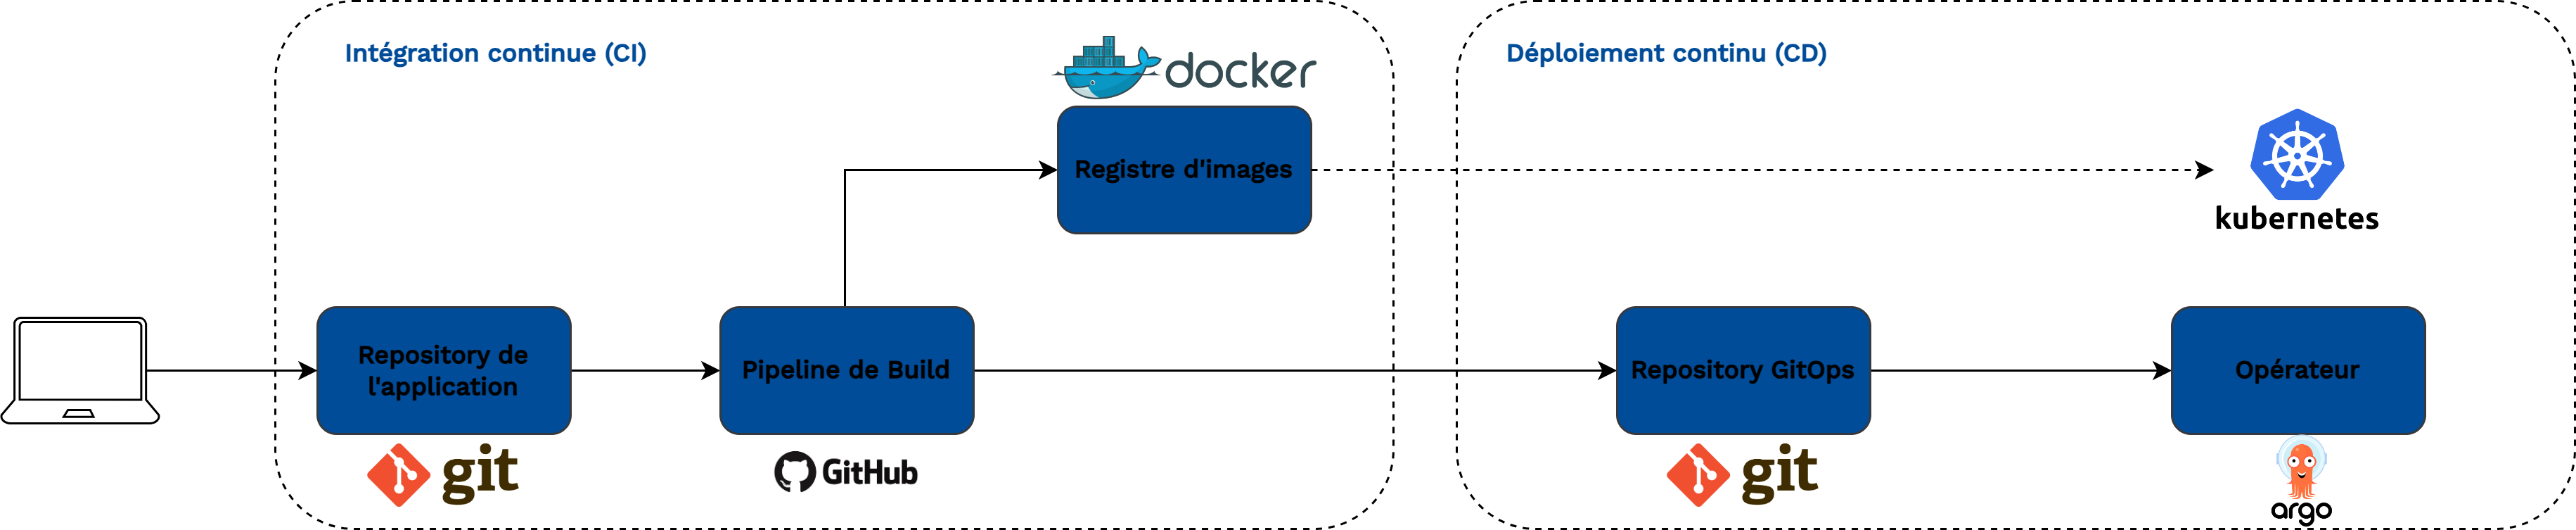
\includegraphics[width=\textwidth]{sections/img/ci-cd.png}
    \caption{Our implementation of a CI/CD pipeline}
    \label{fig:ci-cd}
\end{figure}

\subsubsection{Monitoring a model in production}
\label{subsubsec:monitoring}

Once the modeling phase has been completed, along with training, optimization, and deployment of the model to be accessible to users, it's crucial to understand that the data scientist's responsibilities extend further. Traditionally, the responsibility of the data scientist is often limited to selecting the model to deploy, with the deployment task then delegated to data engineers. However, once in production, the model has not yet reached the end of its lifecycle, and it must be continuously monitored to prevent undesirable performance degradation.

The various components of MLOps, namely data (DataOps), models (ModelOps), and code (DevOps), add complexity to the lifecycle of a ML model by involving multiple stakeholders. Generally, three main actors are involved:

\begin{itemize}
    \item Data scientists/data engineers
    \item IT teams
    \item Business teams
\end{itemize}

Sometimes, data scientists are integrated into business teams and data engineers into IT teams to foster better collaboration. This approach aims to streamline skills, unify terminologies, and align project objectives. In any cases, effective communication remains essential to ensure proper management of the lifecycle of a ML model, particularly concerning monitoring its behavior in a production environment. Continuous monitoring of the deployed model is extremely important to ensure the conformity of results to expectations, anticipate changes in data, and iteratively improve the model. The monitoring is a crucial element of the MLOps approach.

The concept of monitoring can take on different meanings depending on the context of the involved team. For IT teams, it primarily involves verifying the technical validity of the application, including aspects such as latency, memory consumption, or disk usage. Conversely, for data scientists or business teams, the focus is more on methodological monitoring of the model. However, real-time tracking of the performance of a ML model is often a complex task, given that ground truth is usually not known at the time of prediction. Therefore, it is common to use proxies to detect any signs of performance degradation. Two main types of degradation of a ML model are generally distinguished: data drift and concept drift.

\begin{itemize}
    \item \textbf{Data drift}: Data drift occurs when the data used during inference in production exhibits significant differences compared to the data used during training, that is,  $\mathds{P}_{train}(X) \neq \mathds{P}_{inference}(X)$.
    \item \textbf{Concept drift}: Concept drift is evoked when a change in the statistical relationship between the features ($X$) and the target variable ($Y$) is observed over time, that is, $\mathds{P}_{train}(Y|X) \neq \mathds{P}_{inference}(Y|X)$ and $\mathds{P}_{train}(X) = \mathds{P}_{inference}(X)$.
\end{itemize}

In our use case, our objective is to achieve the highest number of correctly classified textual description while minimizing the number of textual description requiring manual intervention. Thus, our goal is to distinguish correct predictions from incorrect ones without prior access to ground truth. To accomplish this, we have developed a confidence index, which represents the difference between the two highest scores. Therefore, for a given textual description, if the confidence index exceeds a determined threshold, the textual description is automatically coded. Otherwise, the textual description is manually coded by an Insee's agent who has access to the five most probable codes according to the model to optimize manual intervention. Defining the threshold for automatic coding of textual descriptions is crucial in production deployment. It involves making trade-offs between achieving a high automatic coding rate and preserving model performance, and vice versa.

To monitor the behavior of our model in production, we have developed an interactive dashboard that enables visualization of several metrics of interest for the business teams. Among these metrics are the number of requests per day and the rate of automatic coding per day based on a given confidence index threshold. This visualization allows business teams to understand the rate of automatic coding they would have obtained if they had chosen different thresholds. It is also possible to visualize the distribution of obtained confidence indices and to compare two temporal windows to determine if there are changes in the distributions of predictions returned by the model\footnote{To compare distributions, you need to calculate the distances between them using, for example the \href{https://en.wikipedia.org/wiki/Bhattacharyya_distance}{Bhattacharyya distance}, the \href{https://en.wikipedia.org/wiki/Kullback\%E2\%80\%93Leibler_divergence}{Kullback-Leibler divergence}, the \href{https://en.wikipedia.org/wiki/Hellinger_distance}{Hellinger distance} or to perform statistical tests such as the \href{https://en.wikipedia.org/wiki/Kolmogorov\%E2\%80\%93Smirnov_test}{Kolmogorov–Smirnov test}, or the \href{https://en.wikipedia.org/wiki/Chi-squared_test}{$\chi^2$-test}.}. 

Confidence indices can be analyzed at finer levels of granularity based on the aggregation level of the nomenclature, to determine which classes are most difficult to predict and which have more or less occurrences. Another part of the dashboard focuses more on the input data of the model and details, for example, the average number of words per textual description, the average number of sentences per textual description, as well as the most frequent words, etc.

% \subsubsection{How to implement a monitoring system in the SSP Cloud?}

Although there are several solutions for monitoring ML models such as \href{https://www.evidentlyai.com/}{Evidently} or \href{https://www.siffletdata.com/}{Sifflet}, we preferred to implement our own solution. Indeed, at the time of our trials, none of the open-source solutions available on the market seemed optimal to us. However, the field of monitoring ML models is still emerging and actively developing, so the statements made today may no longer be true at the time of reading these lines. Before opting, as we did, for an internal solution, we recommend exploring the available tools first.

In our case, we chose to use tools that we already mastered and that seemed suitable for our problem. We thus used DuckDB for optimized management of our data and the Dashboard feature of Quarto for creating the interactive dashboard. 

First, to monitor in real-time the activities of your API, it is essential to integrate logs, whether to monitor technical or methodological aspects. We made the decision, which may be subject to debate, to include \textit{business information} such as the output code and its corresponding confidence index in the API logs. The objective was to be able to build our dashboard based on the logs returned by the API. To exploit these logs, we set up a kind of Extract-Transform-Load (ETL) process in Python, which retrieves the API logs and transforms them into partitioned parquet files exploitable by the dashboard. Ideally, we would have preferred to rely on a tool capable of performing this parsing natively and more structured than us. \href{https://www.parseable.com/}{Parseable} could have been such a solution, but unfortunately, it was not installable on the SSP Cloud for technical reasons. We then use Quarto and its Dashboard feature to create an interactive dashboard. The various metrics present in the dashboard are calculated by making SQL queries directly on our parquet files with DuckDB. The dashboard is deployed in the same way as our API, that is, in a container based on an image that is automatically built via Github Actions as soon as the code associated with the dashboard is modified. Figure \ref{fig:monitoring-datalab} depicts the setup of our monitoring system, highlighting the various technologies employed.

In summary, our monitoring pipeline consists of:

\begin{enumerate}
    \item Including \textit{business logs} in the API for every request.
    \item Utilizing ArgoCD to schedule a nightly ETL job, generating partitioned parquet files stored on MinIO.
    \item Employing ArgoCD for continuous deployment, where the dashboard dynamically retrieves data from the parquet file via DuckDB, computes metrics, and offers interactive visualization.

\end{enumerate}

\begin{figure}[htbp]
    \centering
    \makebox[\textwidth][c]{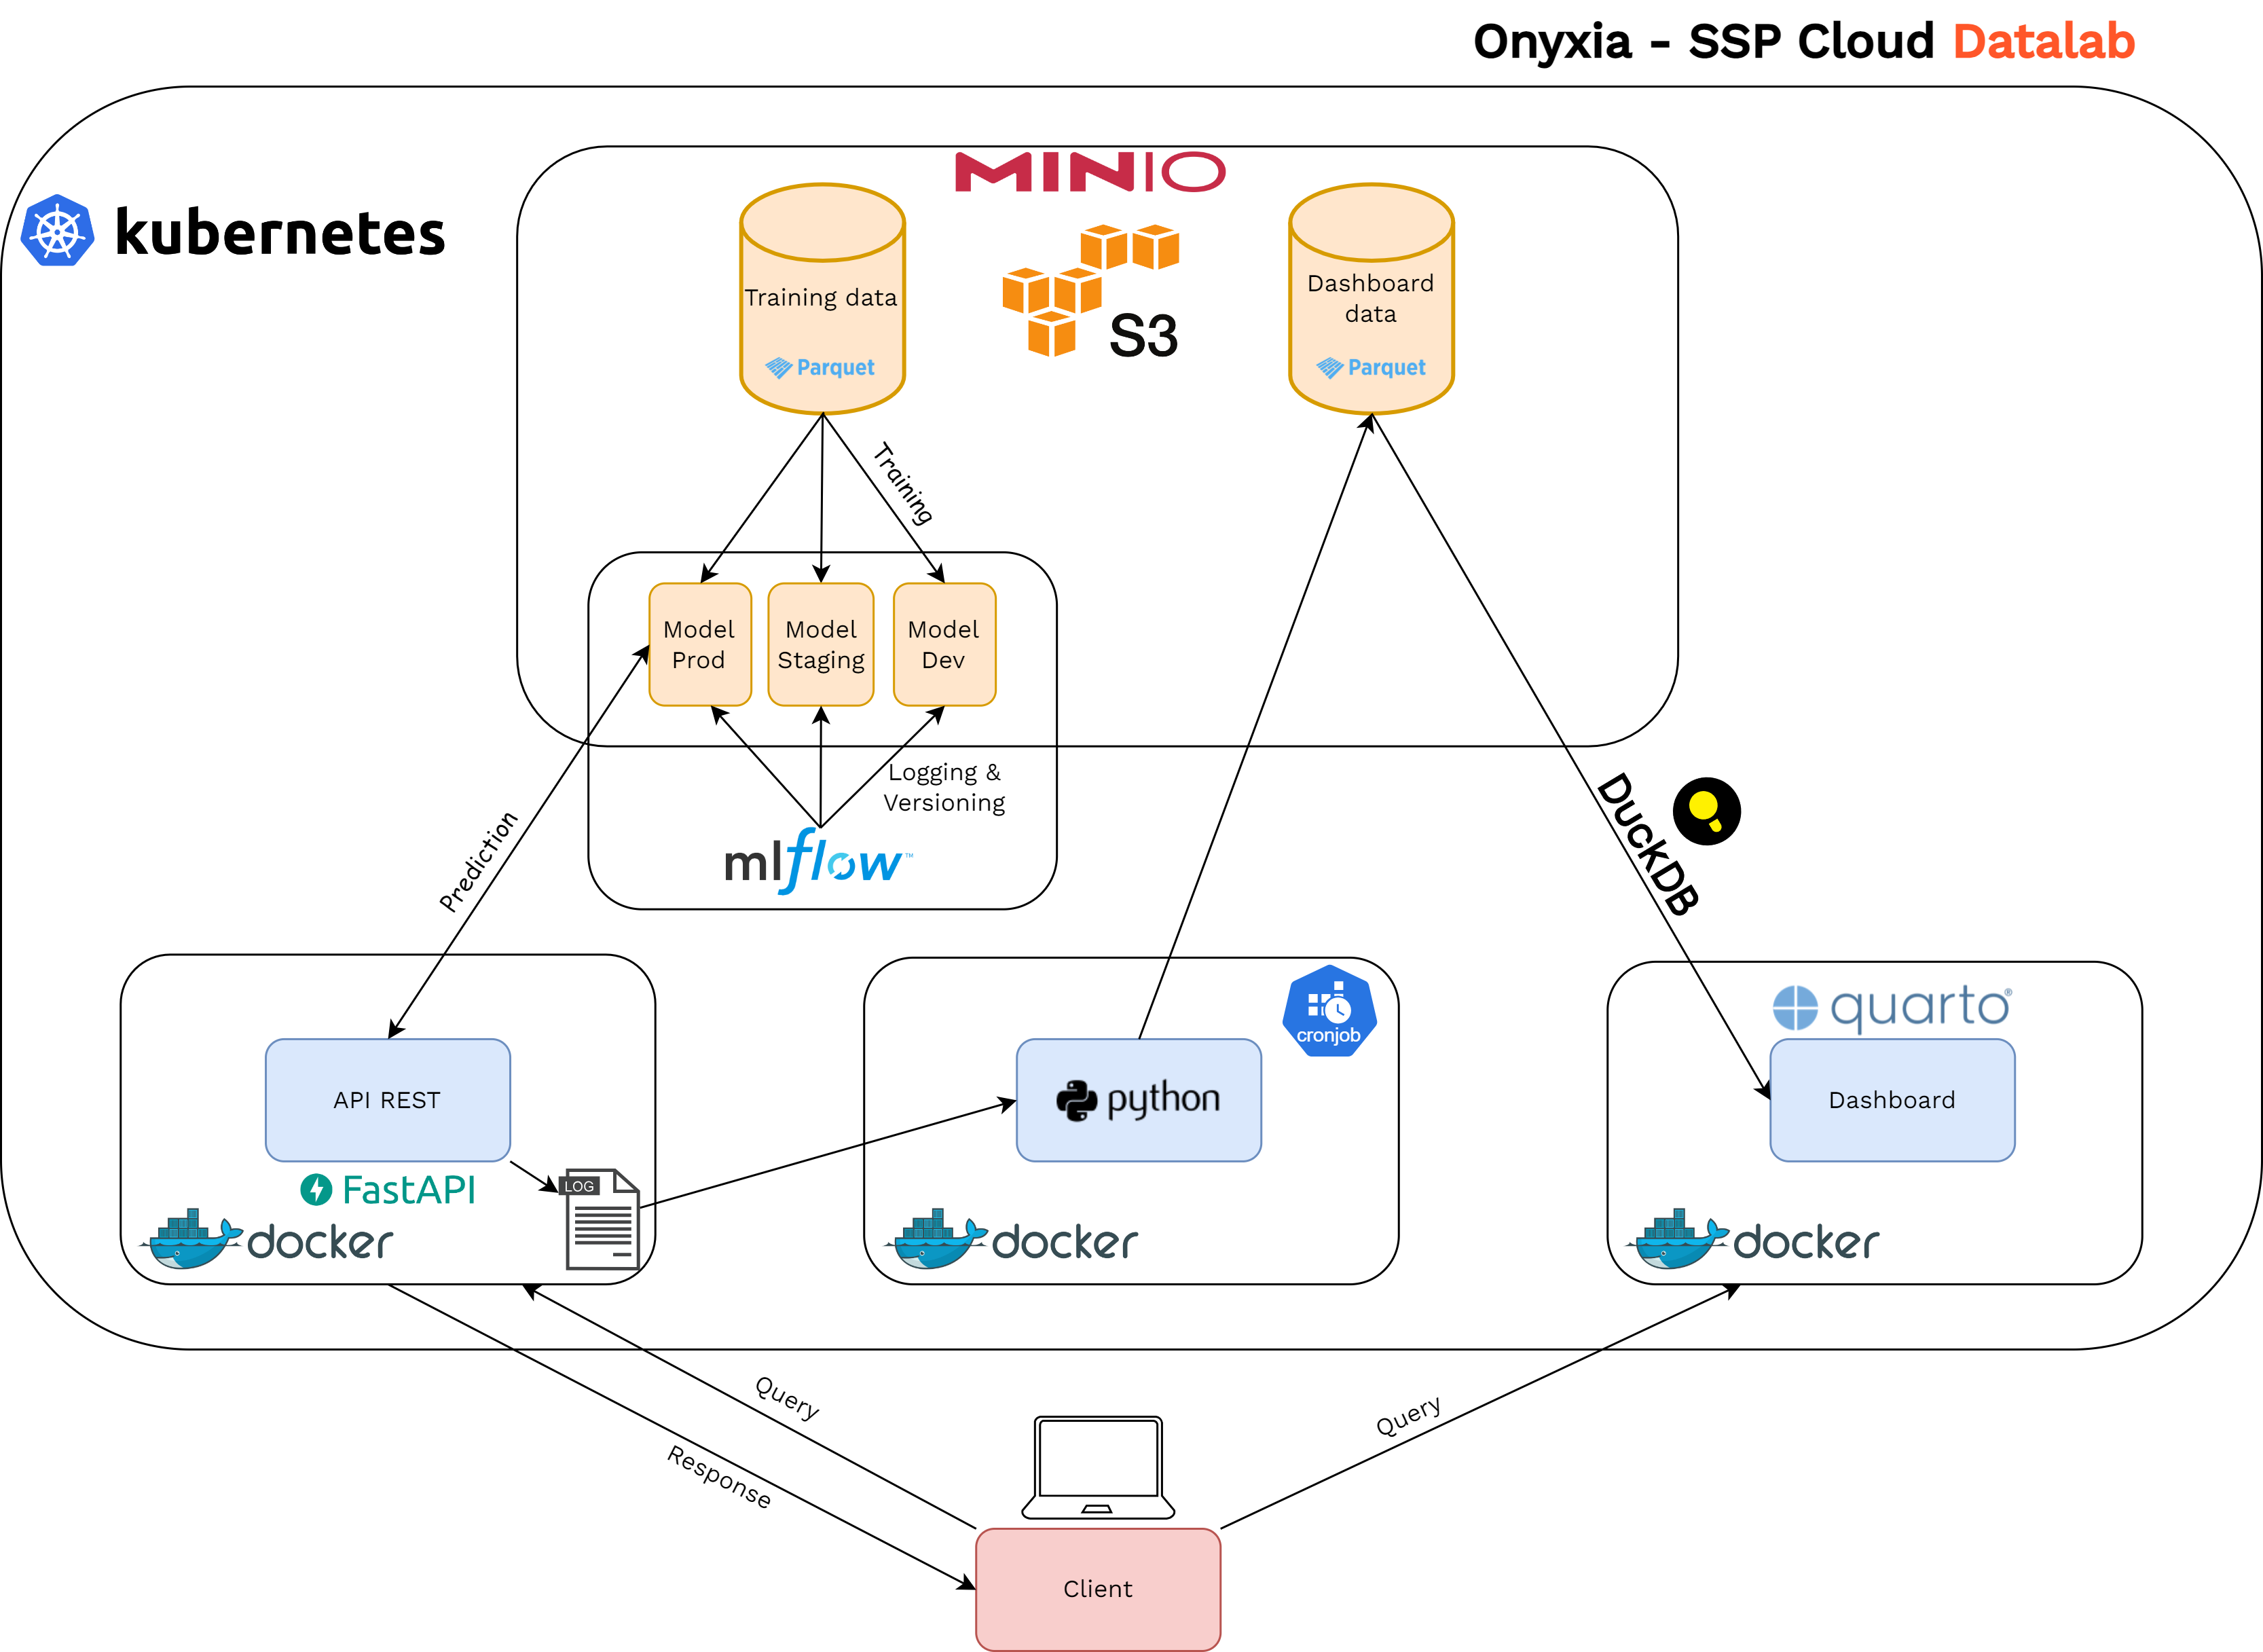
\includegraphics[width=1.5\textwidth]{sections/img/monitoring-datalab.png}}
    \caption{In-house implementation of a monitoring system}
    \label{fig:monitoring-datalab}
\end{figure}


\subsubsection{Promoting continuous improvement of the model}
\label{subsubsec:annotation}

In all ML projects, it is well-established that data is key, and in supervised ML problems, annotations play a crucial role in model performance. At the project's onset, time constraints compelled us to swiftly achieve results, precluding the luxury of conducting a comprehensive annotation campaign. Consequently, we never had access to a truly annotated gold-standard test sample on which we could rely 100\%. To evaluate the performance of our model, we relied on a subset of our training dataset (test/train split), knowing that its labeling was not perfect. After several months of model deployment, it became imperative to build such a gold-standard test sample. Firstly, this sample allows us to have an unbiased view of the model's performance in production on real data, particularly on data that has been automatically coded. Additionally, this sample enabled us to identify and correct inconsistencies present in our initial training dataset. 

Convincing the business teams of the significance of annotation proved challenging, as they were reluctant to reallocate new human resources, which necessitated specialized expertise, on a tedious task. However, the model's increased automation in coding enabled the teams to shift their focus to annotation tasks.


Another reason that motivated the implementation of annotation campaigns is the redesign of the NACE nomenclature in 2025. From 2025 onwards, European statistical institutes will be required to use the latest version of NACE, namely NACE Rev. 2.1. This revision brings substantial changes that will require retraining a new model. For this, a new training dataset with the correct annotations is peremptory. A back-propagation work on the old training dataset is also considered to increase the size of the dataset. Thus, a dual annotation campaign was initiated in early 2024 on the SSP Cloud platform.

To carry out these annotation campaigns, we used the \href{https://labelstud.io/}{Label Studio} service, available on the SSP Cloud. Label Studio is an open-source platform designed to facilitate data annotation. The first annotation campaign aims to create a test dataset allowing continuous evaluation of our model and improvement of the training dataset if necessary. To do this, we create a pool of text descriptions randomly sampled from the data passed through the API over the past three months. This sample is then sent to annotation by NACE experts using the UI of Label Studio. The annotation results are automatically saved on MinIO, transformed into parquet format, and then integrated into the monitoring dashboard to compute and observe various model performance metrics. The second annotation campaign is dedicated to the transition to the new version of NACE. The objective is to allocate certain experts to annotation in the new version of NACE to create a training dataset for the future model. In this revision, some codes are univocal, meaning for example that code 0112Z will become 0112Y, while others are multivocal, such as 0119Z, which can become either 0113Y or 0119Y. The challenge lies primarily with the latter, which is why, to streamline this annotation process, only the textual descriptions of multivocal codes are sent for annotation on Label Studio.

Once again, the presence of a cloud-native technology on the platform, such as Label Studio, allowed us to swiftly kickstart this annotation campaign while seamlessly integrating it with the various components of our architecture, as depicted in Figure \ref{fig:annotation-datalab}.

\begin{figure}[htbp]
    \centering
    \makebox[\textwidth][c]{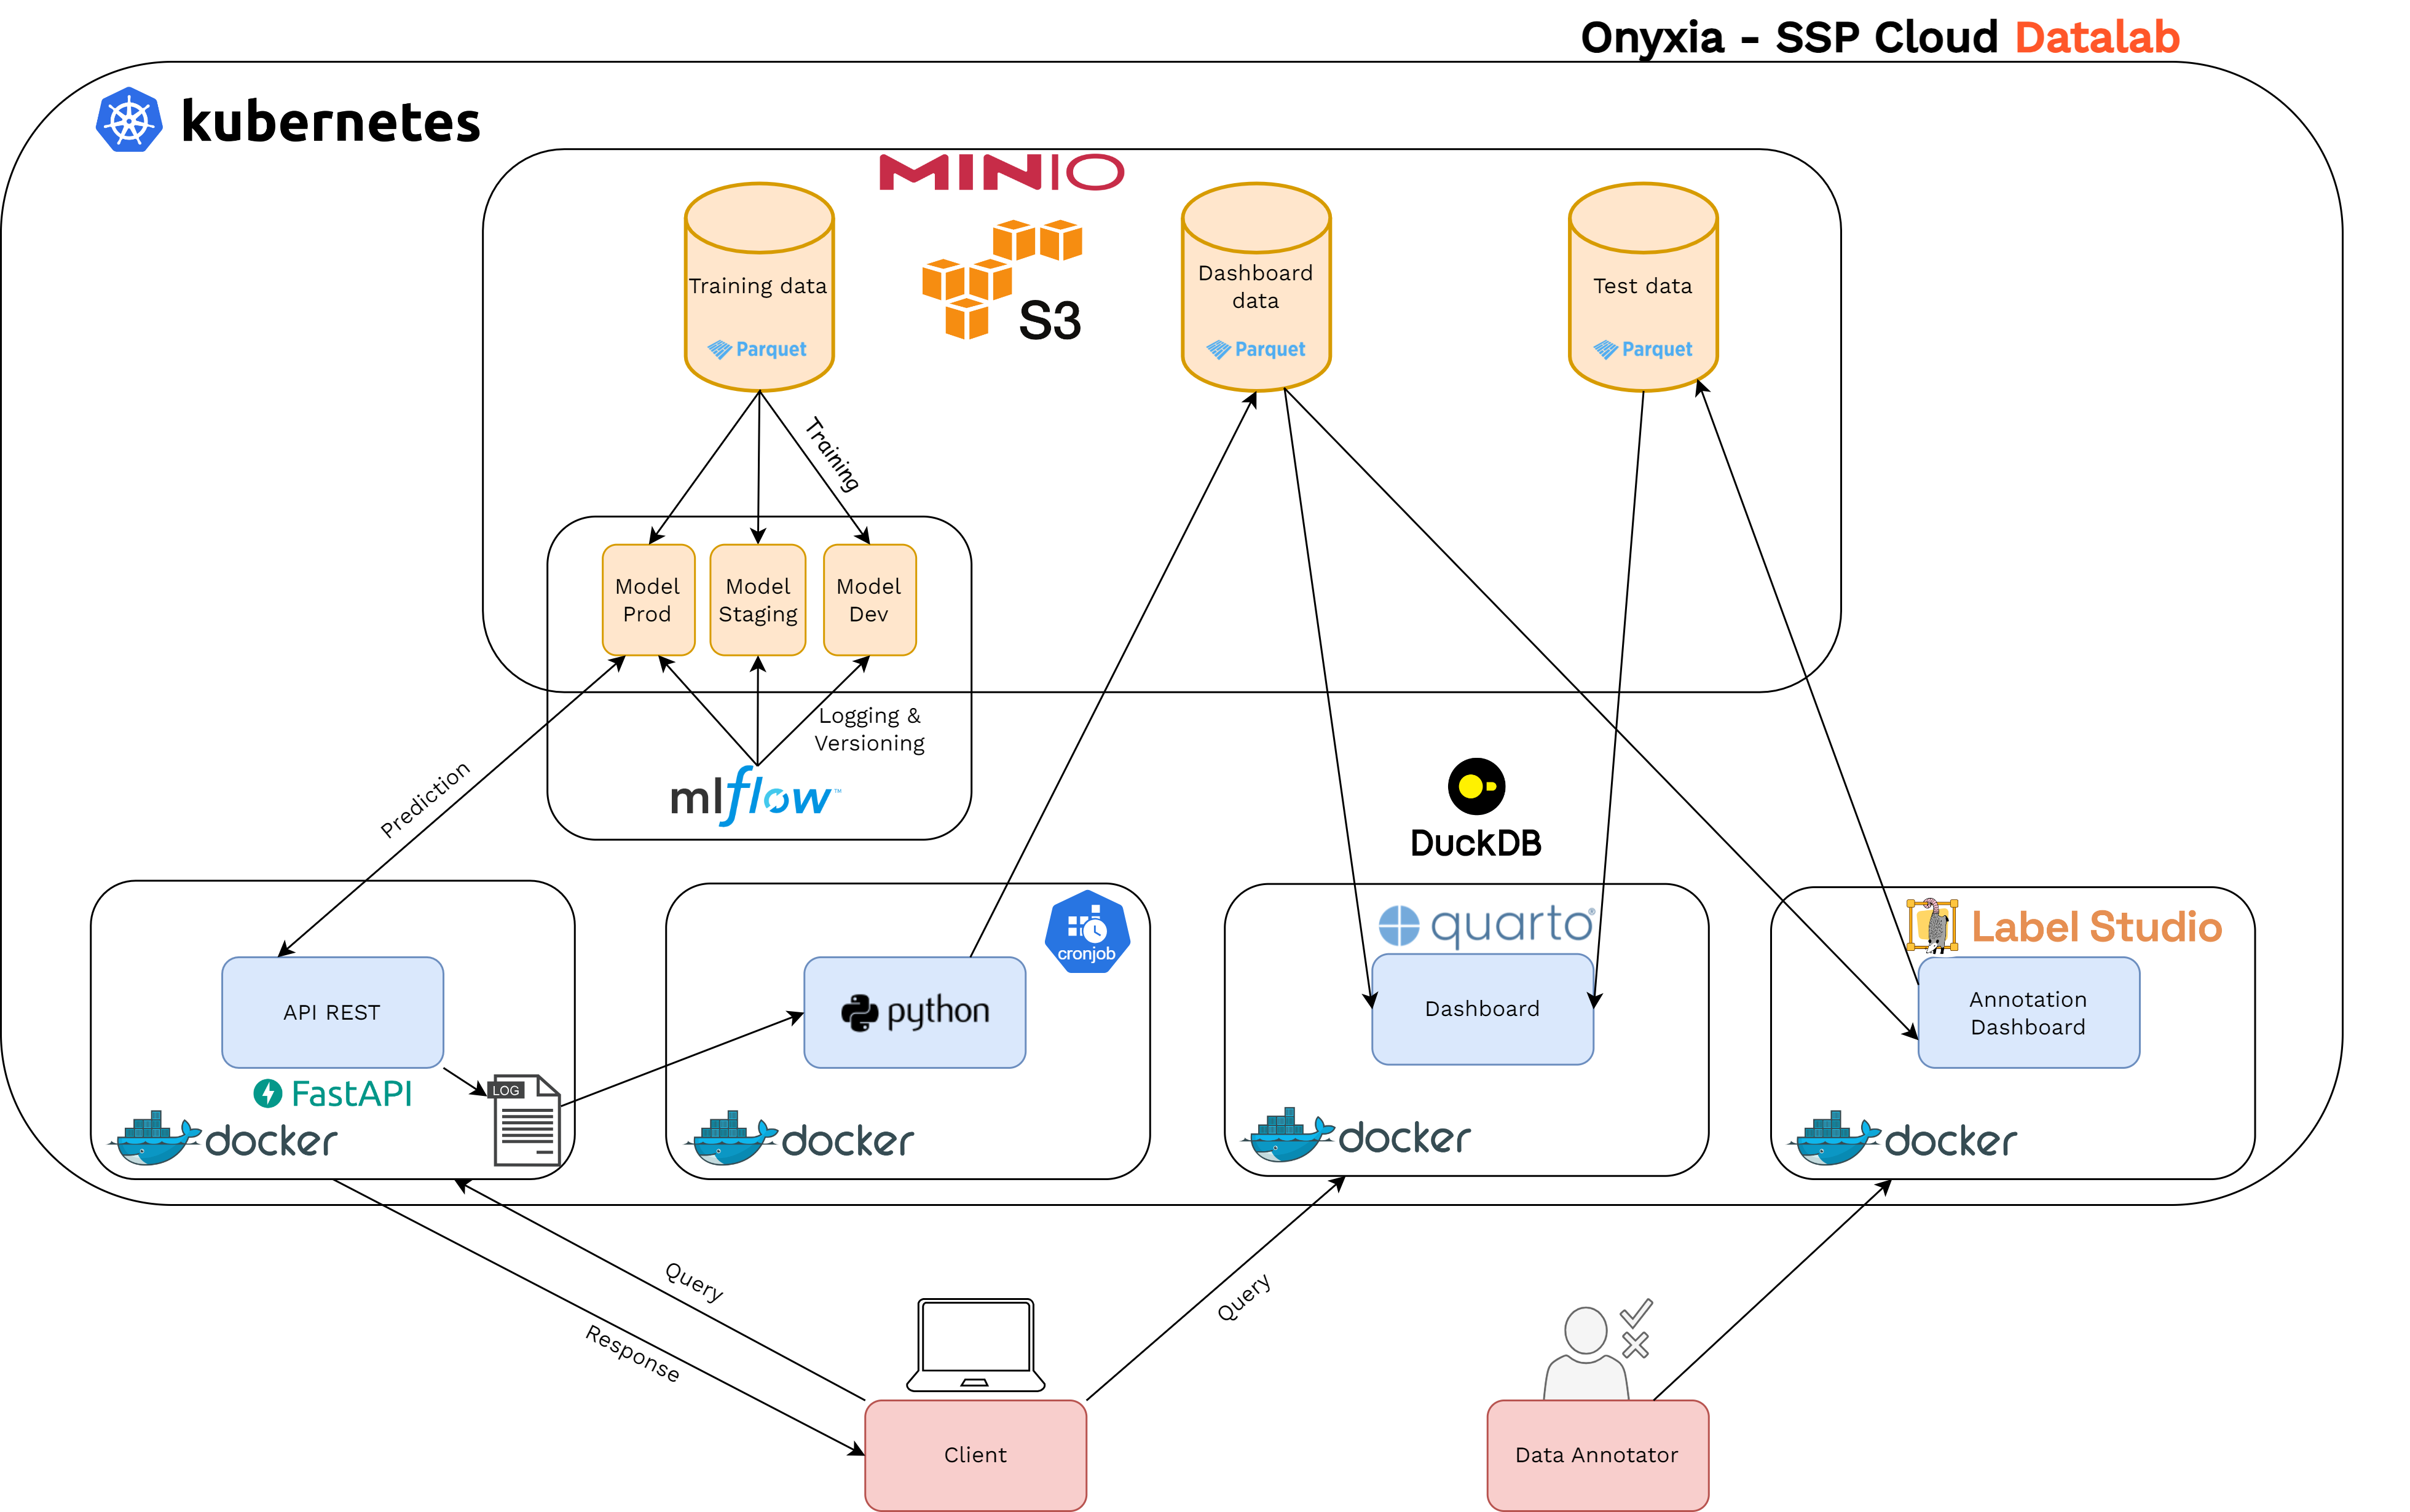
\includegraphics[width=1.5\textwidth]{sections/img/annotation-datalab.png}}
    \caption{Implementation of data quality control using Label Studio}
    \label{fig:annotation-datalab}
\end{figure}


\label{sec:5}
\section{Discussion}

\subsection{Future}

\begin{itemize}
    \item Onyxia, un bien commun opensource largement réutilisé (Insee, SSB) $\rightarrow$ faciliter les contributions pour la postérité du projet open-source, qui dépasse l'Insee
    \item One-stop-shop : SSP Cloud comme plateforme de référence pour les projets de ML $\rightarrow$ croissance de l'offre de formation (+ traduction)
    \item Accompagner les réinstanciations (datafid, POCs dans le secteur privé)
    \item Multiplication des projets qui passent en prod (applications de dataviz, modèles de ML avec MLOps, webscraping : Jocas/WINs)
\end{itemize}

\subsection{Discussion}

\begin{itemize}
    \item Cout d'entrée important pour l'organisation : stockage objet, cluster kube/conteneurisation
    \begin{itemize}
        \item Choix fondamental d'archi $\rightarrow$ limite à la diffusion d'onyxia
        \item Assumer le choix : compétences, organisation~...
        \item Mais globalement : tendance favorable car beaucoup d'orga et INS font ce choix
    \end{itemize}
    \item Cout d'entrée important pour le statisticien :
    \begin{itemize}
        \item Non-persistence de l'environnement $\rightarrow$ git + stockage objet
        \item Travail dans un conteneur $\rightarrow$ perte de repères sur l'environnement
        \item Mais formation : bonnes pratiques + écoles de formation Insee + accompagnements
    \end{itemize}
    \item SSP Cloud :
    \begin{itemize}
        \item Instance ouverte $\rightarrow$ absence de données sensibles $\rightarrow$ grosse limitation des cas d'usage réalisables + frustrations $\rightarrow$ en résumé, difficile de maximiser à la fois innovation et sécurité (pb sur-contraint)
        \item $\rightarrow$ résolution via le choix de l'innovation max car sujet des échanges inter-administration de données complexe + le SSP Cloud a pavé la voie à des instances internes, plus fermées $\rightarrow$ stratégie assumée "platform-as-a-package" : projet open-source packagé $\rightarrow$ facilité ++ de réinstanciation
        \item Pas une plateforme de diffusion de données $\rightarrow$ pas de stratégie globale de gouvernance $\rightarrow$ le sujet de la méta-donnée n'est pas abordé.
    \end{itemize}
    \item Gouvernance :
    \begin{itemize}
        \item Quelle organisation ? Equipe DS centralisée qui vient en appui ou data scientists dans les orgas métiers ? Collaboration avec les équipes infos ? (cf. graphique orga/compétences de Romain)
    \end{itemize}
\end{itemize}


\section*{Appendix}
\addcontentsline{toc}{section}{Appendix}
%
%

\bibliographystyle{plain}
\bibliography{refs}

\end{document}
